\documentclass{beamer}

\useoutertheme[subsection=false]{miniframes}
\usecolortheme{beaver}
\setbeamertemplate{navigation symbols}{}
\setbeamertemplate{footline}{}
\usepackage{graphicx}
\usepackage{url}
\usepackage{datetime}
\usepackage{tikz-cd}
\newcommand{\lectureDate}{\formatdate{08}{11}{2018}}

\setbeamertemplate{caption}
{\raggedright\insertcaption\par}
\title{MATH211: Linear Methods I}
\author{Matthew Burke}
\date{\lectureDate}
\begin{document}

\frame{\titlepage}

\begin{frame}{Lecture on \lectureDate}
  \tableofcontents
\end{frame}

\section*{Last time}
\label{sec:Last-time}

\begin{frame}{Last time}
  \begin{itemize}
  \item Complex numbers\vfill
  \item Addition of complex numbers\vfill
  \item Multiplication of complex numbers\vfill
  \item Division of complex numbers
  \end{itemize}
\end{frame}

\section{Graphical interpretation}

\begin{frame}
\begin{beamercolorbox}[sep=12pt,center]{part title}
\usebeamerfont{section title}
\insertsection\par
\end{beamercolorbox}
\end{frame}

\begin{frame}[fragile]{Graphical interpretation}
Consider the function $\mathbb{R} \rightarrow \mathbb{R}$ that multiplies by $-1$:
\begin{equation*}
\begin{tikzcd}[column sep=0.2cm]
&\dots&-x&\dots& -2 & -1  & 0 & +1& +2 & \dots&x\arrow[bend right, color = blue, leftrightarrow]{llllllll}&\dots&\\
\end{tikzcd}
\end{equation*}
which shows us that $-1\times(-1\times x) = x$.\vfill
(Imagine this as a rotation rather than reflection.)
\end{frame}

\begin{frame}[fragile]{Graphical interpretation}
So how do we get a transformation that squares to $-1$?
\begin{equation*}
\begin{tikzcd}
{} & {} & +i & {} & {}\\
-2 & -1 & 0 & +1 \arrow[bend right, color = blue]{ul} & +2\\
\end{tikzcd}
\end{equation*}
\end{frame}

\begin{frame}[fragile]{Graphical interpretation}
So how do we get a transformation that squares to $-1$?
\begin{equation*}
\begin{tikzcd}
{} & {} & +i \arrow[bend right, color = blue]{dl} & {} & {}\\
-2 & -1\arrow[bend right, color = blue]{dr} & 0 & +1 \arrow[bend right, color = blue]{ul} & +2\\
{} & {} & -i\arrow[bend right, color = blue]{ur} & {} & {}
\end{tikzcd}
\end{equation*}
\end{frame}

\begin{frame}[fragile]{Graphical interpretation}
\begin{columns}
	\column{0.5\textwidth}
	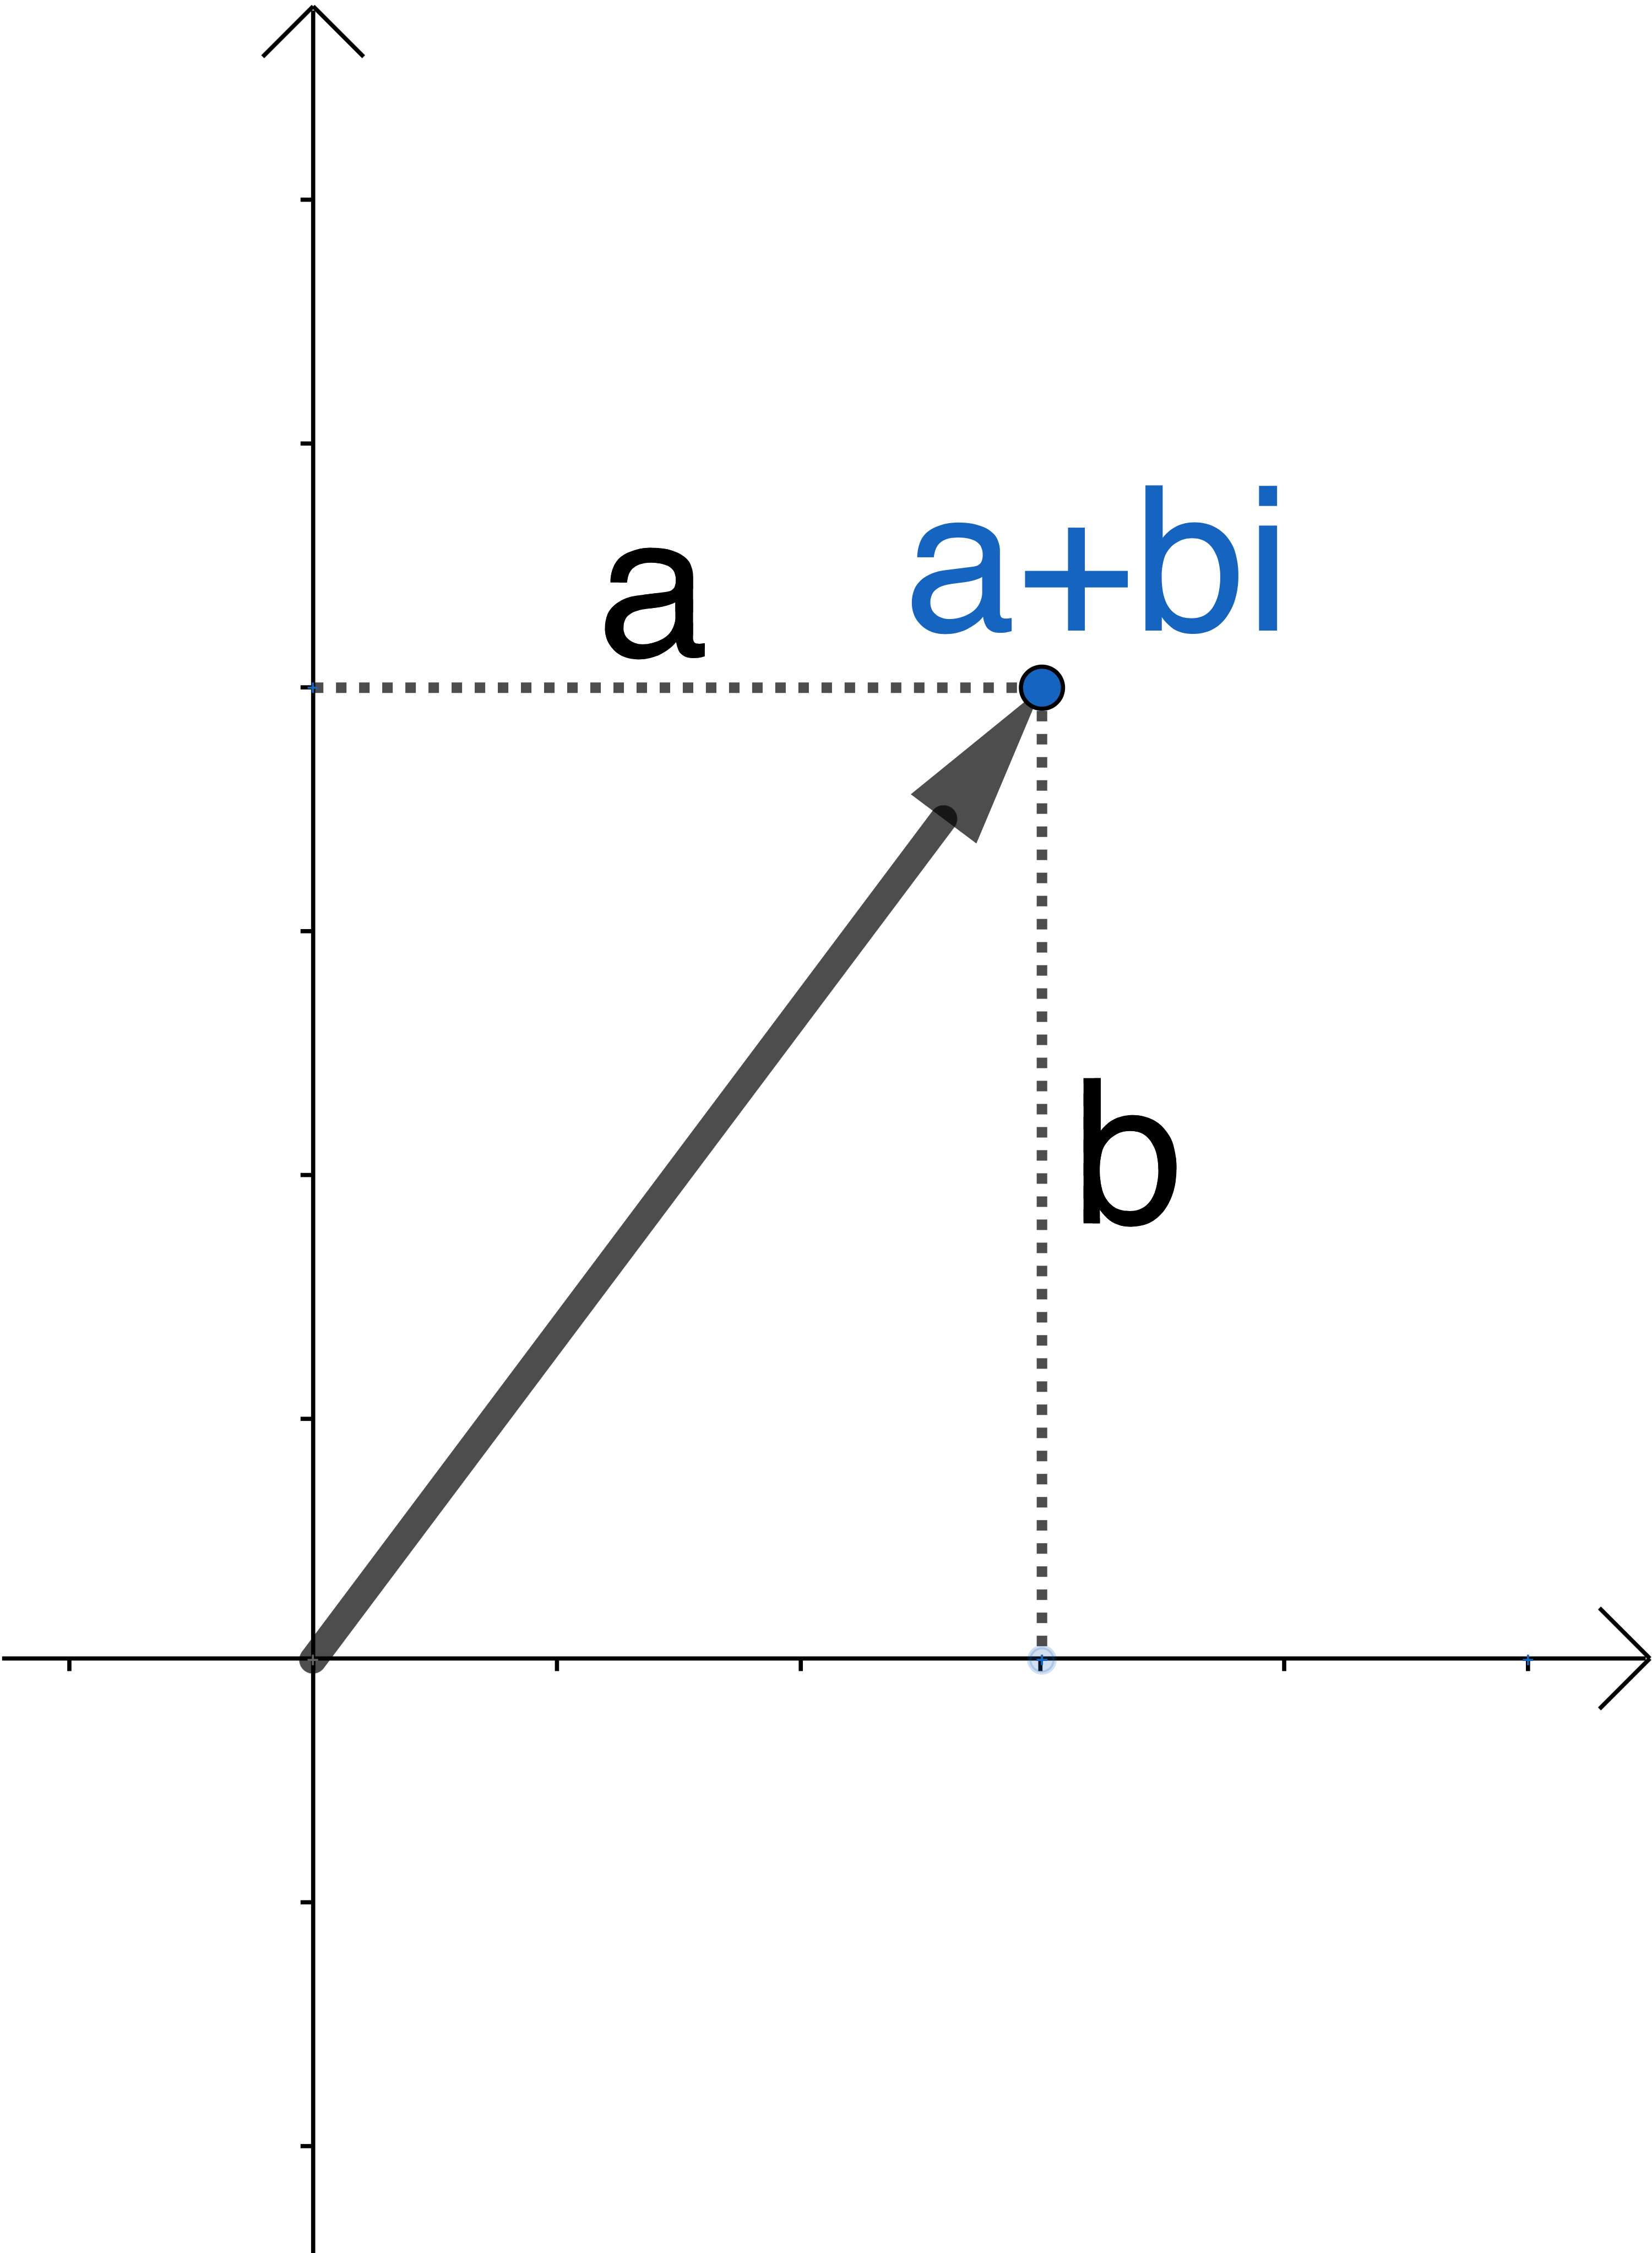
\includegraphics[scale=0.8]{complex-plane.png}
	\column{0.4\textwidth}
	We draw the complex number $z=a+bi$ as the point $(a, b)$ in $\mathbb{R}^2$.\vfill
	\begin{definition}
	The \emph{modulus of $z$} is its length in $\mathbb{R}^2$:
	\begin{equation*}
	|z| = \left| \left[
	\begin{array}{c}
	a\\
	b
	\end{array}
	\right]\right| = \sqrt{a^2+b^2}
	\end{equation*}
	\end{definition}
\end{columns}
\end{frame}

\begin{frame}{Addition of complex numbers}
\begin{columns}
\column{0.4\textwidth}
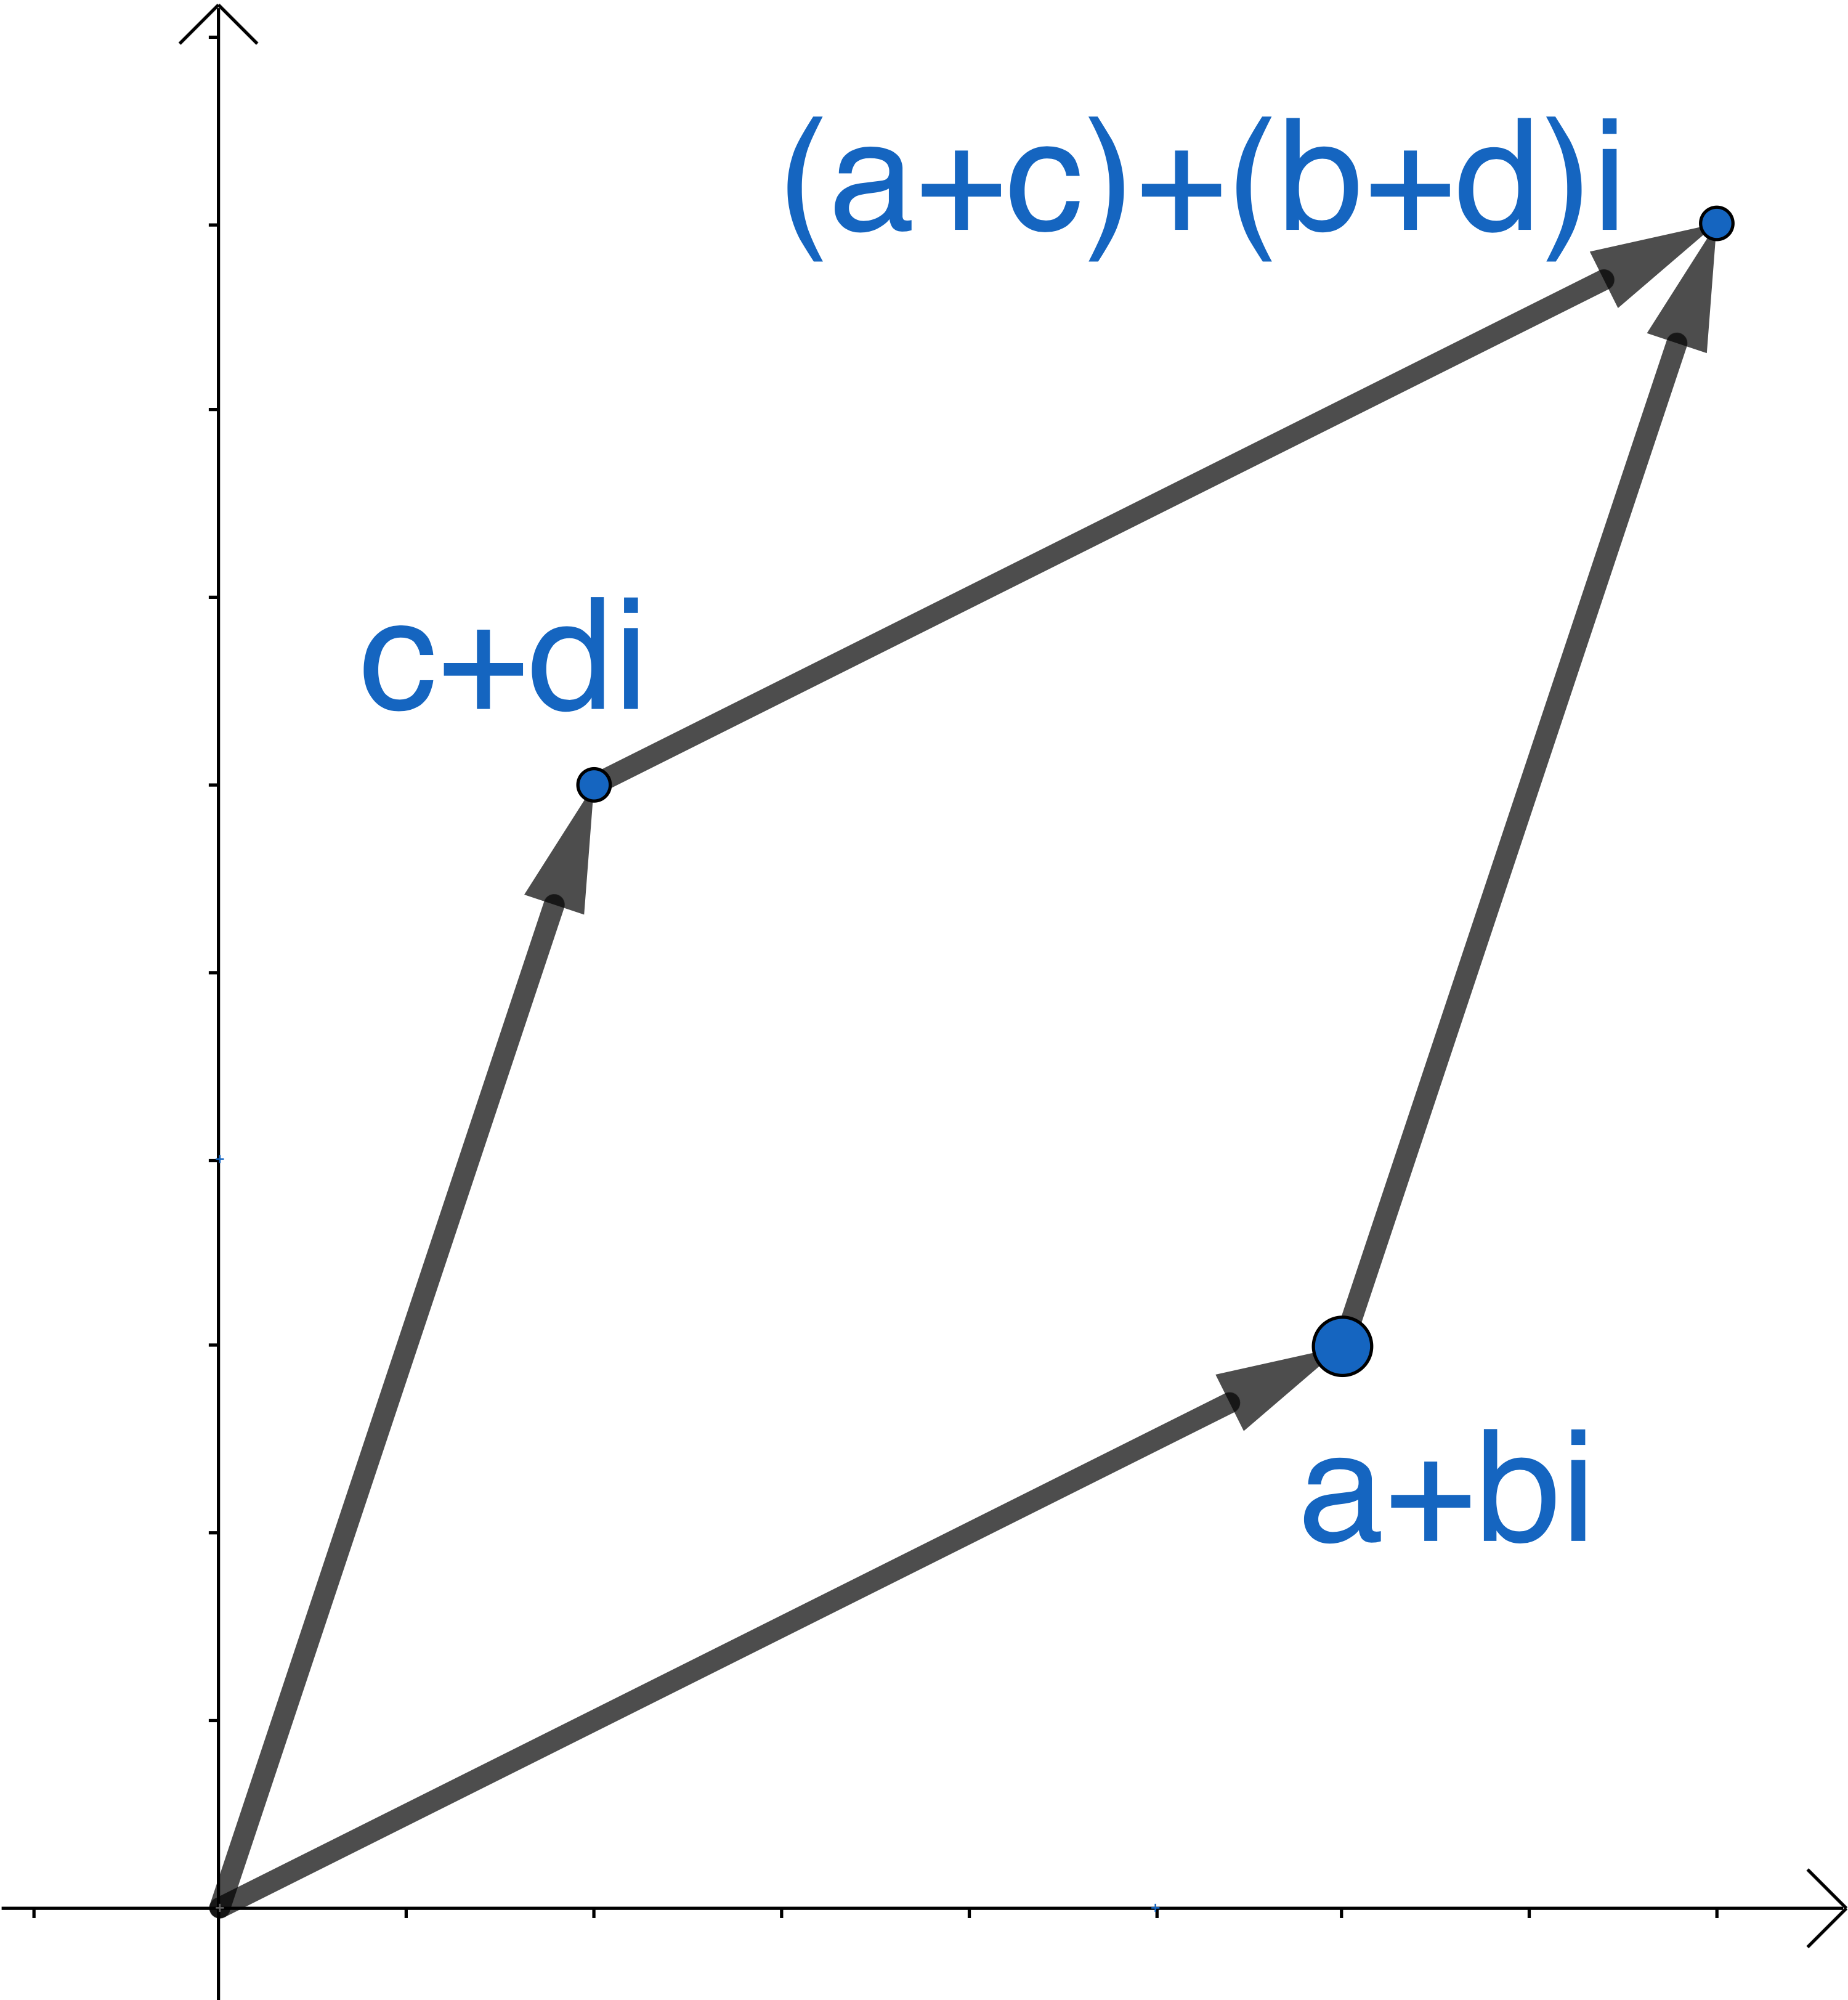
\includegraphics[scale=0.5]{complex-addition.png}
\column{0.5\textwidth}
Complex addition is defined component-wise:
\begin{equation*}
(a+ib)+(c+id) = (a+c)+(b+d)i
\end{equation*}
and therefore has the same graphical interpretation as the addition of vectors in $\mathbb{R}^2$.
\end{columns}
\end{frame}

\begin{frame}{Graphical interpretation of multiplication}
Next section.
\end{frame}

\begin{frame}{Conjugate}
\begin{columns}
	\column{0.5\textwidth}
	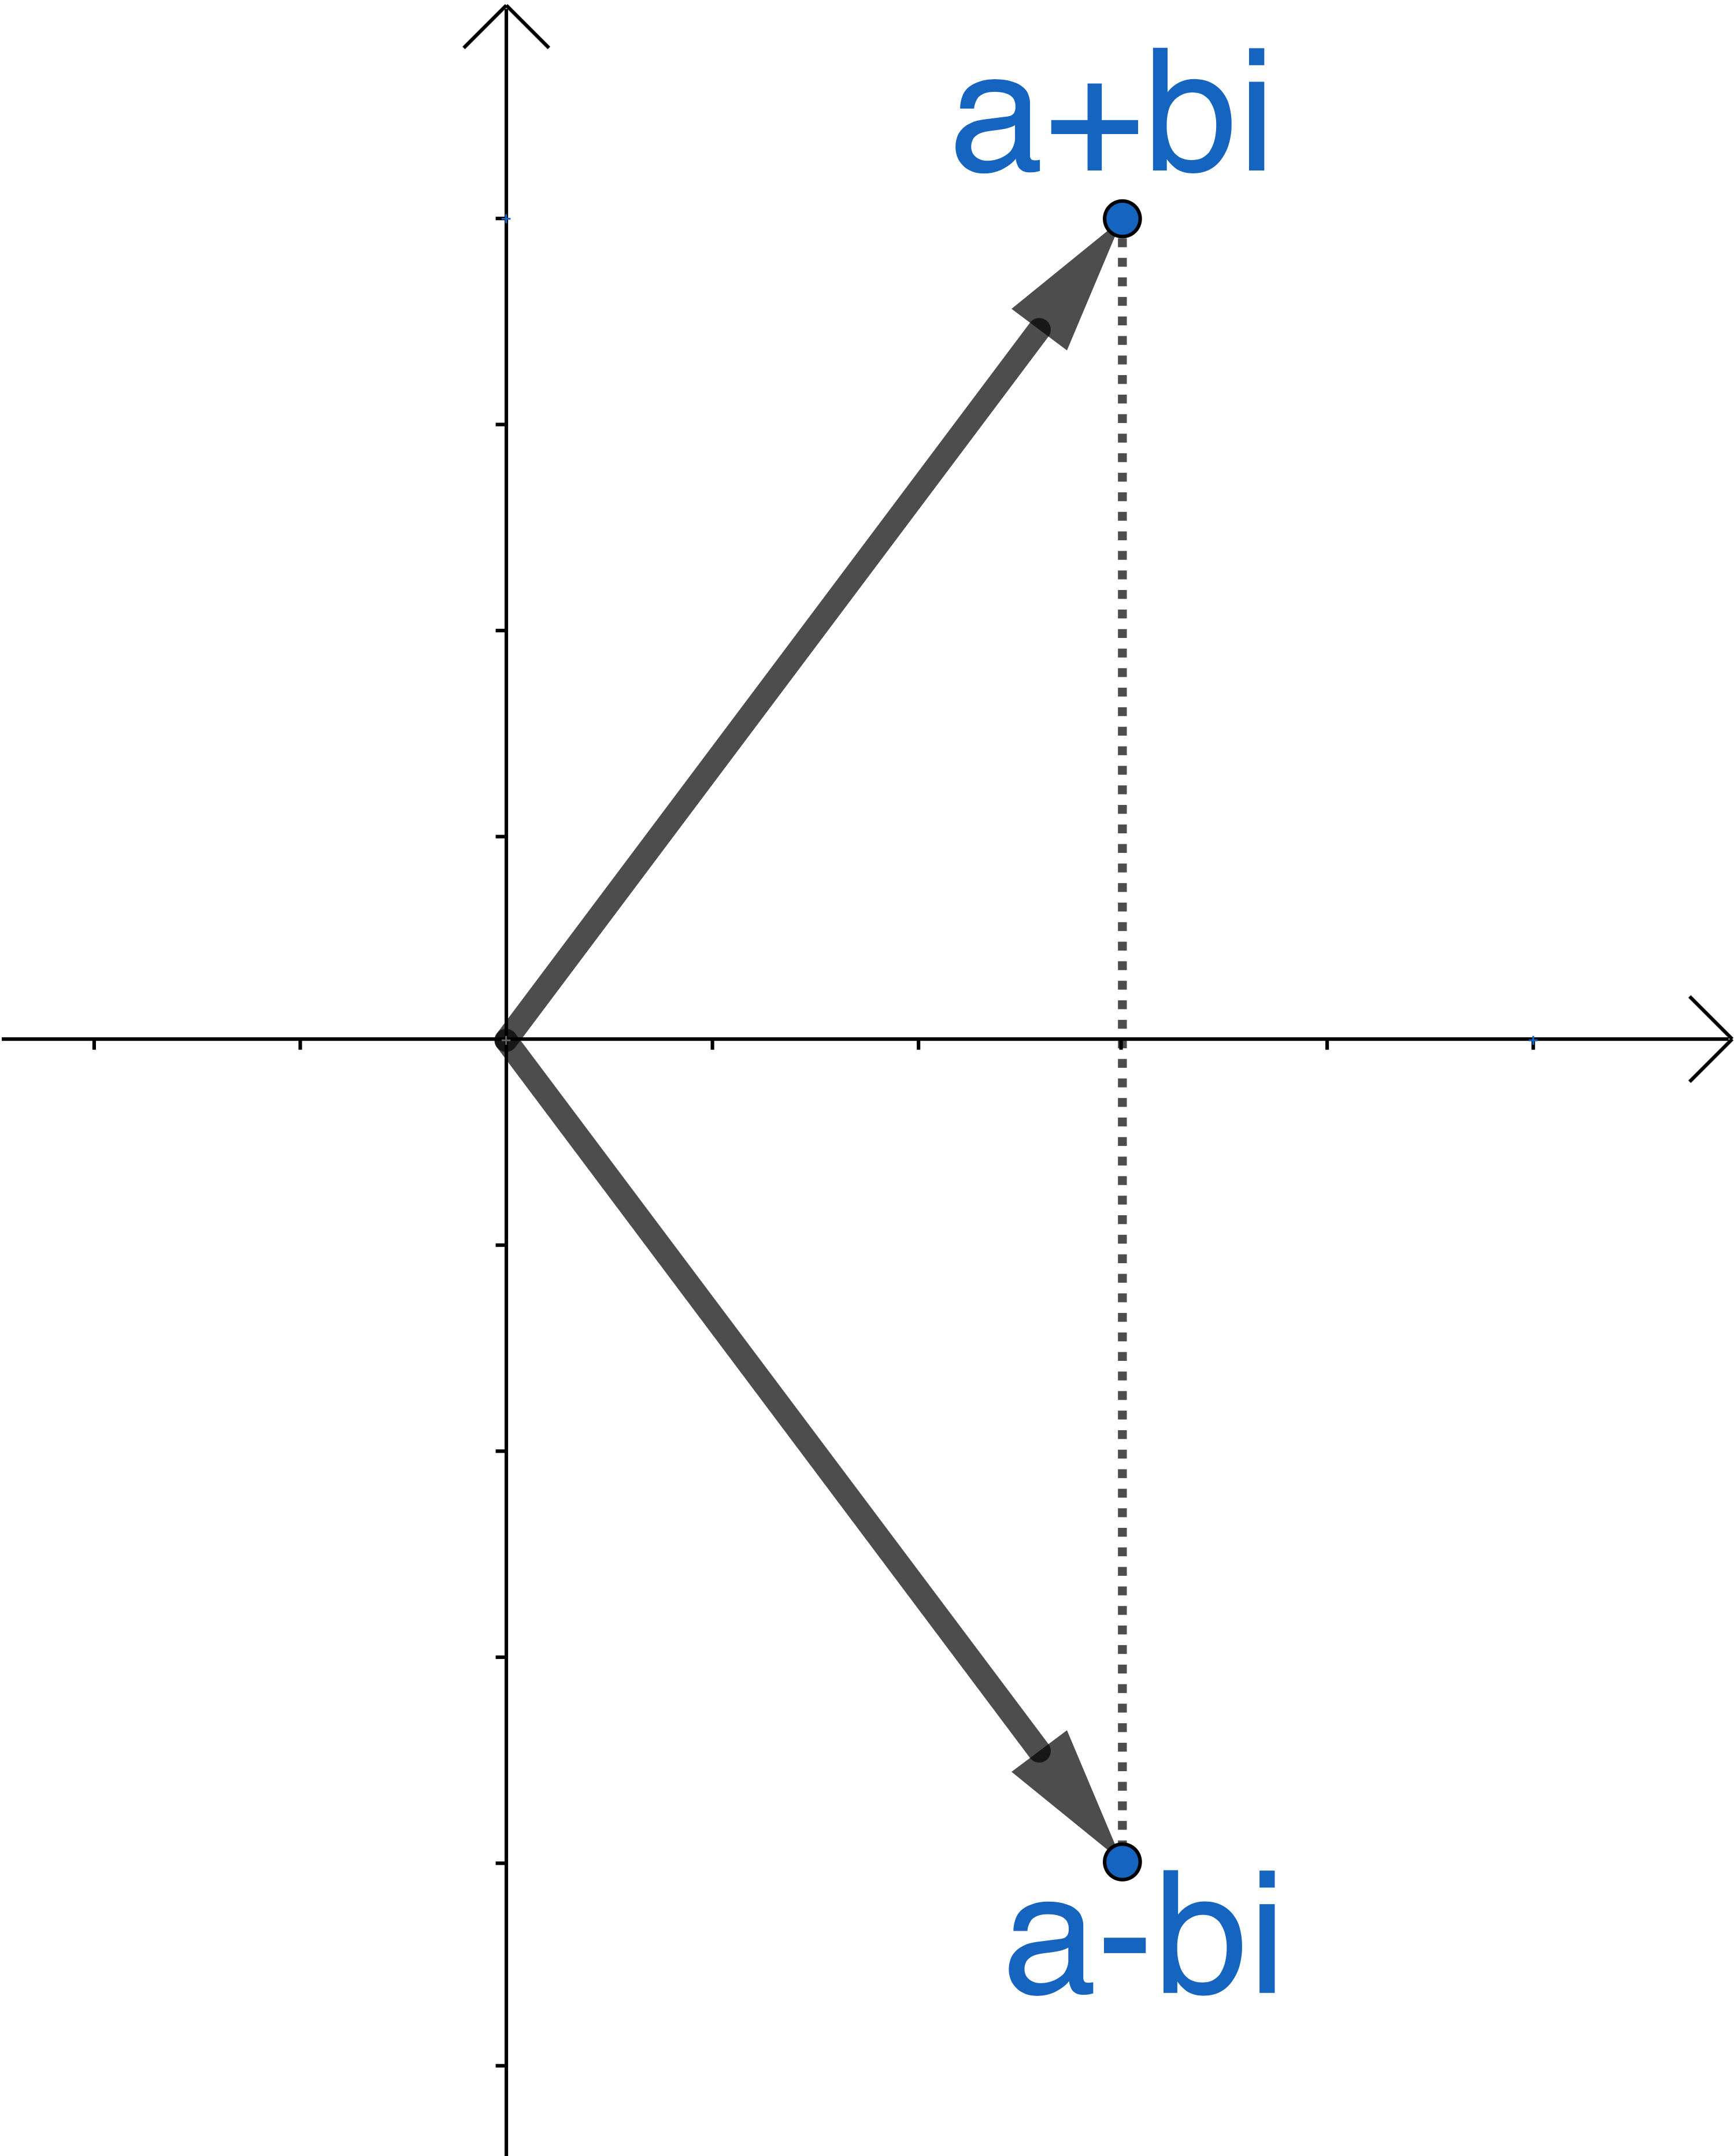
\includegraphics[scale=0.6]{conjugate.png}
	\column{0.4\textwidth}
	\begin{definition}[Conjugate]
	If
	\begin{equation*}
	z=a+bi
	\end{equation*}
	then
	\begin{equation*}
	\overline{z} = a-bi
	\end{equation*}
	\end{definition}
\end{columns}
\end{frame}

\begin{frame}{Properties of conjugate}
Let $z$ and $w$ be complex numbers.
\begin{itemize}
\item
$\overline{z\pm w} = \overline{z} \pm \overline{w}$.
\item
$\overline{(zw)} = \overline{z}~ \overline{w}$.
\item
$\overline{(\overline{z})}=z$.
\item
$\overline{\left(\frac{z}{w}\right)} =
\frac{\overline{z}}{\overline{w}}$.
\item
$z$ is real if and only if $\overline{z}=z$.
\end{itemize}
If $z=a+bi$, then
\[ z\overline{z}=
(a+bi)(a-bi)=
a^2 + b^2=|z|^2\]
\end{frame}

\begin{frame}{Questions?}
Questions?
\end{frame}

\begin{frame}{Examples}
\begin{example}
	\begin{itemize}
		\item $|-3+4i|$
		% ANS: 5
		\item $|3-2i|$
		% ANS: sqrt(13)
		\item $|i|$
		% ANS: 1
	\end{itemize}
\end{example}
\begin{example}
\begin{itemize}
\item $\overline{3+4i}$
\item $\overline{-2+5i}$
\item $\overline{i}$
\item $\overline{7}$
\end{itemize}
\end{example}
\end{frame}

\section{Polar form}

\begin{frame}
\begin{beamercolorbox}[sep=12pt,center]{part title}
\usebeamerfont{section title}
\insertsection\par
\end{beamercolorbox}
\end{frame}

\begin{frame}{Polar co-ordinates}
\begin{columns}
\column{0.5\textwidth}
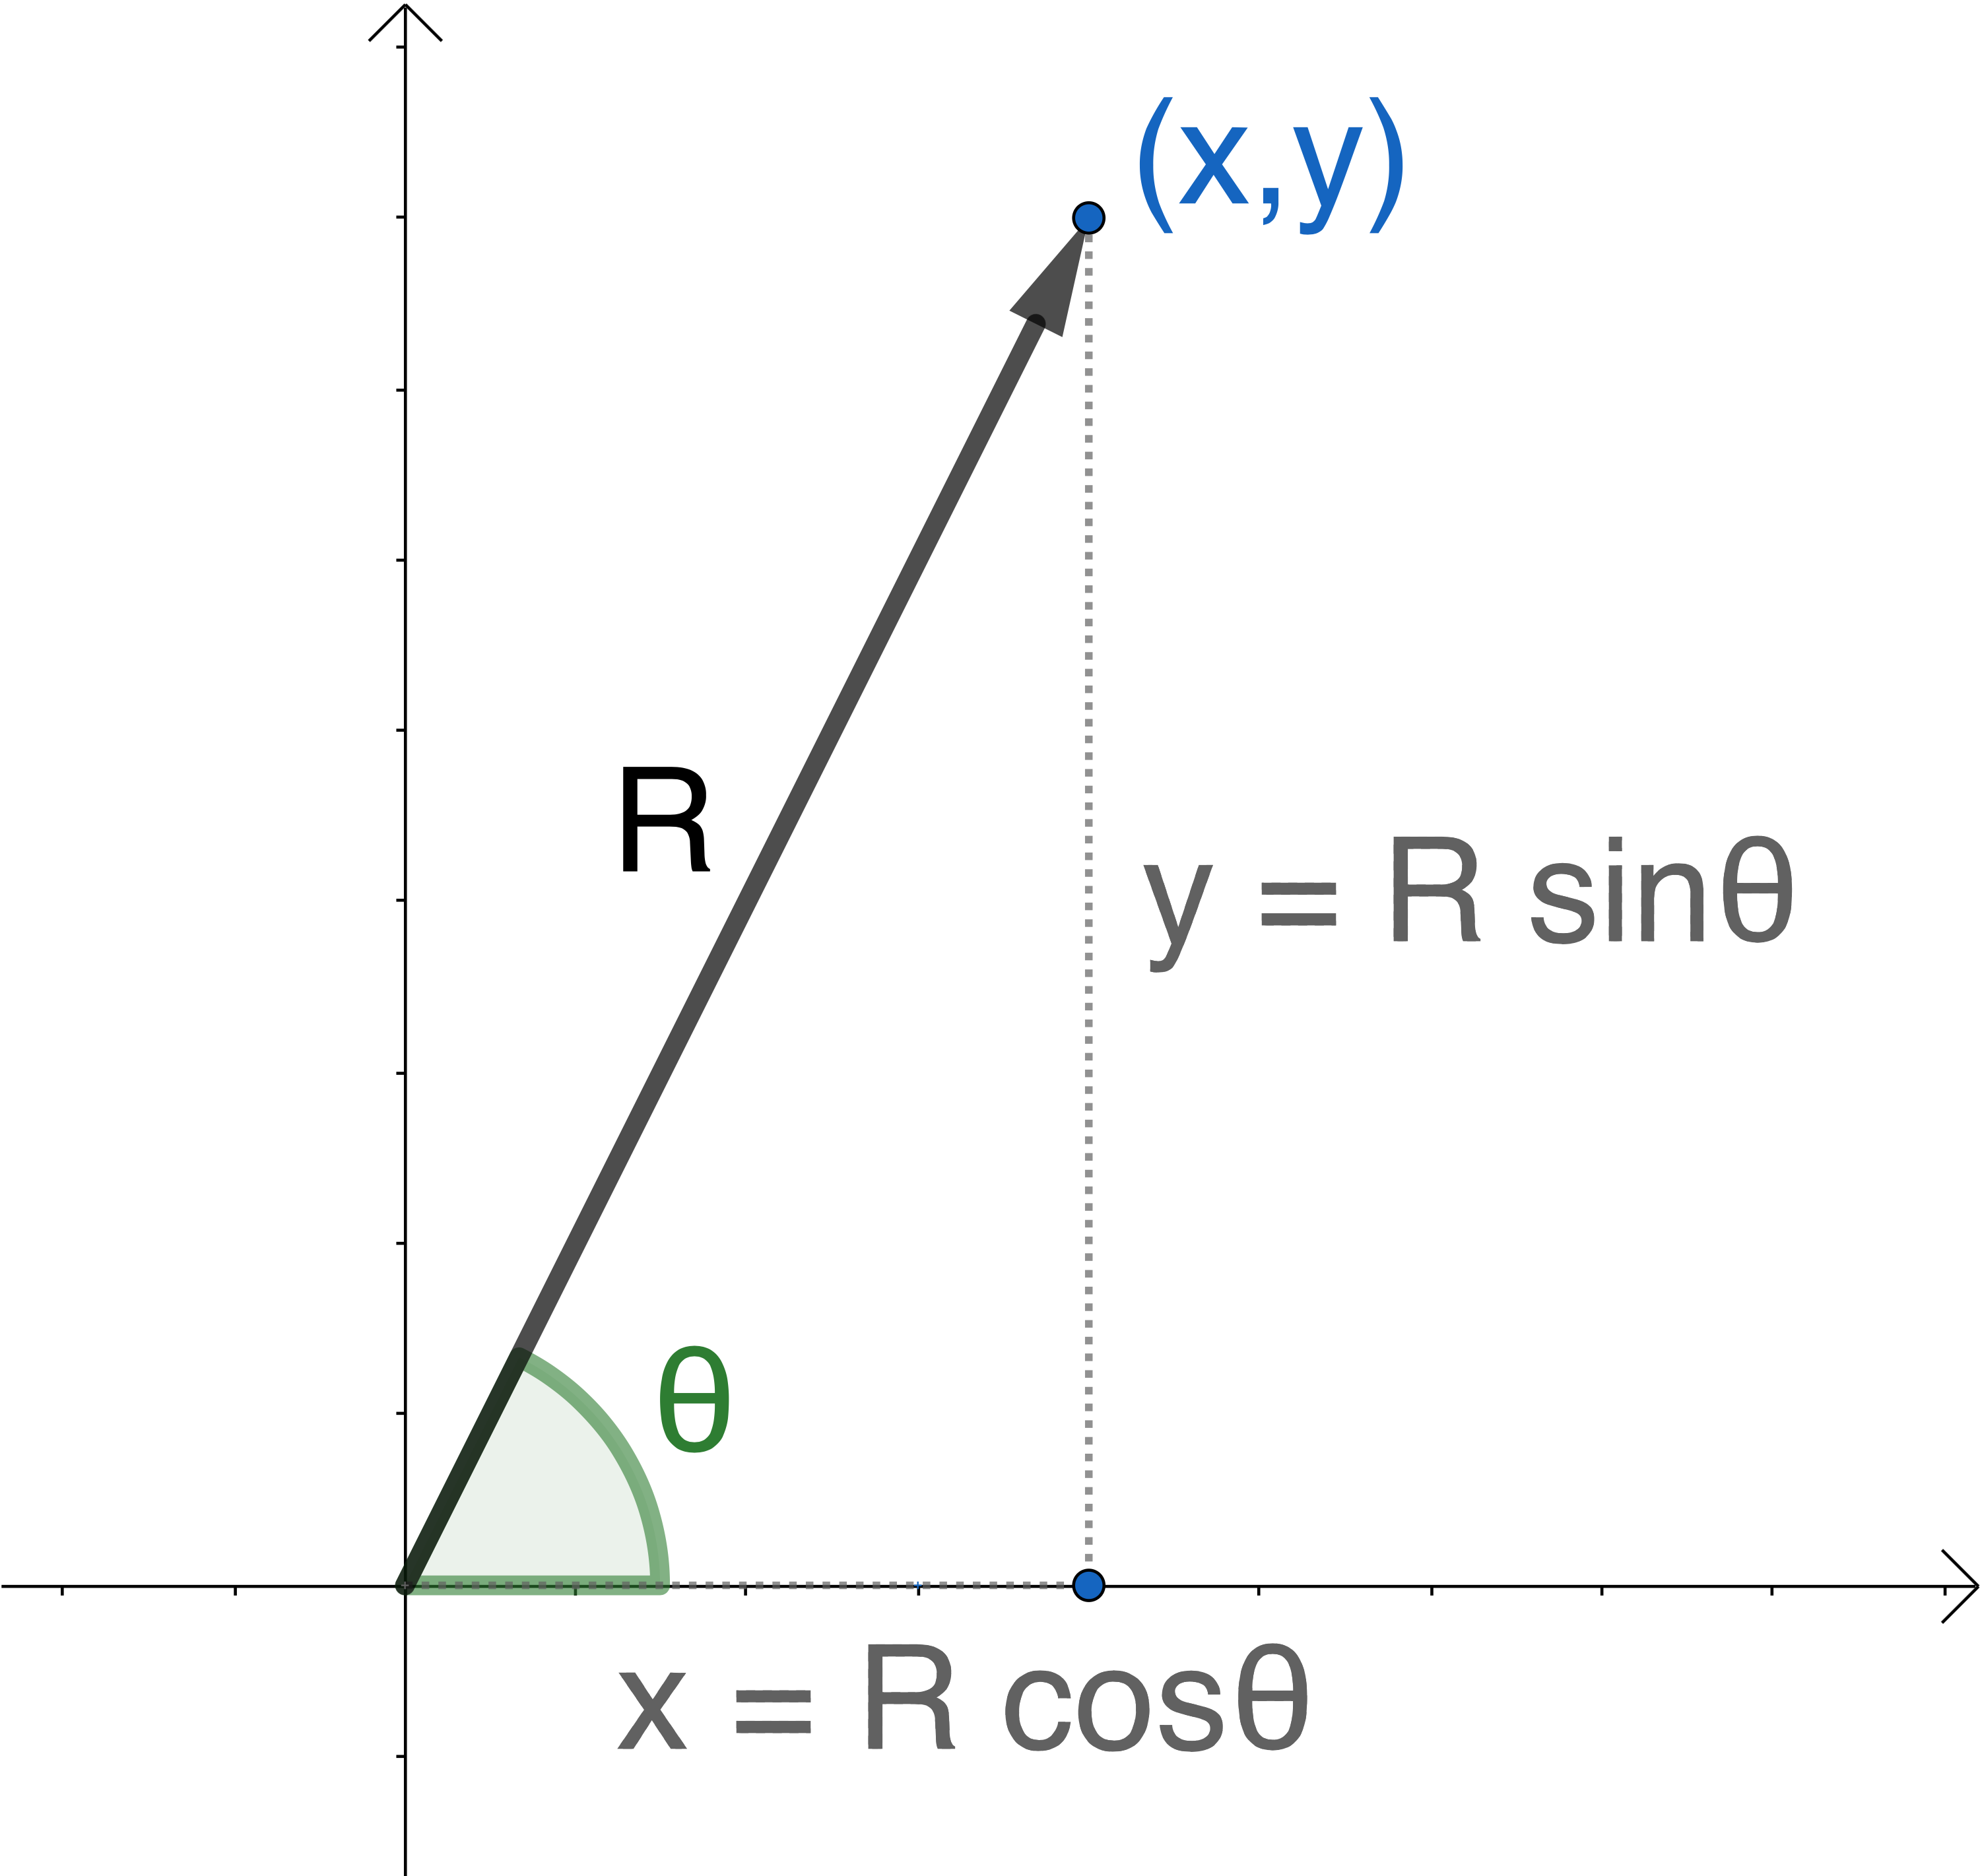
\includegraphics[scale=0.55]{polar-form.png}
\column{0.4\textwidth}
We can describe a point in the plane in terms of an angle and magnitude.
By convention we let $\theta$ range between
\begin{equation*}
-\pi< \theta \leq +\pi
\end{equation*}
and if $R=0$ we say the angle is undefined.
\end{columns}
\end{frame}

\begin{frame}{Converting from polar to Cartesian}
\begin{columns}
\column{0.5\textwidth}
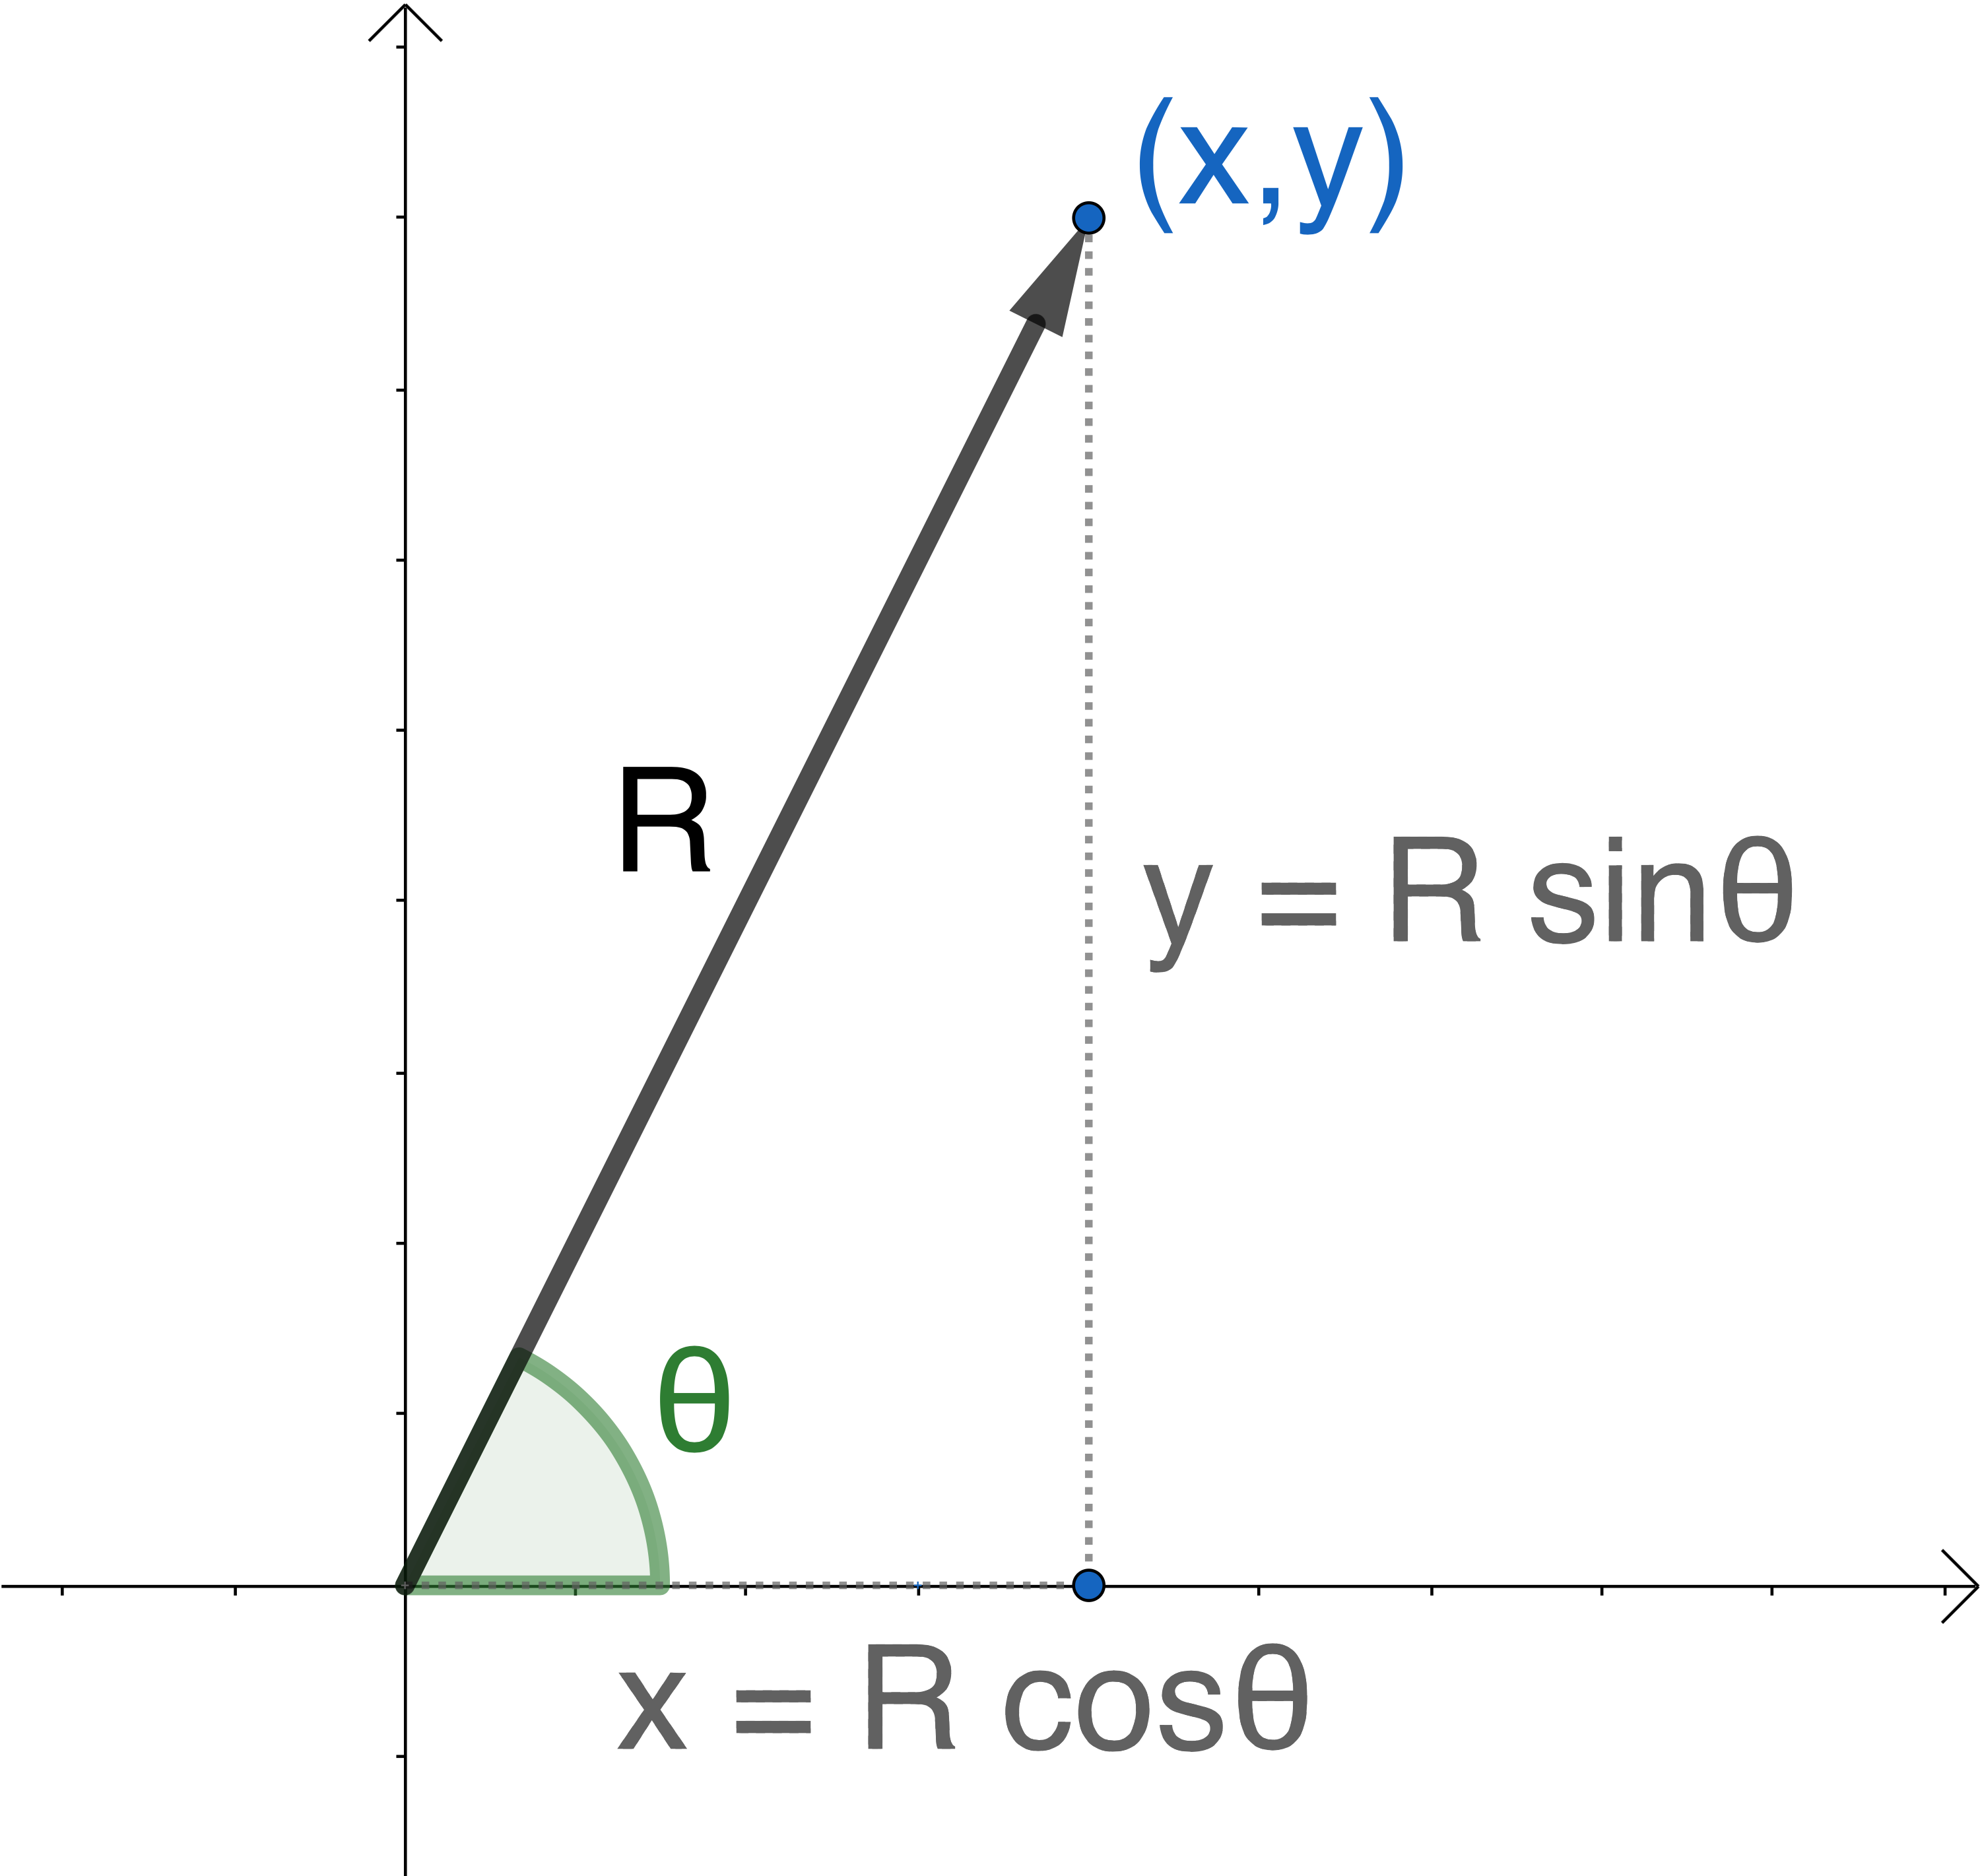
\includegraphics[scale=0.55]{polar-form.png}
\column{0.4\textwidth}
If we have $R$ and $\theta$ then:
\begin{align*}
	x &= R \cos\theta\\
	y &= R \sin\theta
\end{align*}
(and if $R=0$ then $x=0$ and $y=0$).\vspace{0.5cm}
\end{columns}
\end{frame}

\begin{frame}{Examples}
\begin{example}
\begin{itemize}
	\item $(1, 0)$ has $R=1$ and $\theta = 0$.
	\item $(0,1)$ has $R=1$ and $\theta = \frac{\pi}{2}$.
	\item $(0,-1)$ has $R=1$ and $\theta = \frac{-\pi}{2}$.
	\item $(1, 1)$ has $R = \sqrt{2}$ and $\theta = \frac{\pi}{4}$.
	\item $(1, \sqrt{3})$ has $R=2$ and $\theta = \frac{\pi}{3}$.
\end{itemize}
\end{example}
\end{frame}

\begin{frame}{Converting from Cartesian to polar}
If we are given Cartesian co-ordinates $(x, y)$ then
\begin{equation*}
R = \sqrt{x^2+y^2}
\end{equation*}
and we would like to use
\begin{equation*}
\theta = \tan^{-1}\left(\frac{y}{x}\right)
\end{equation*}
but unfortunately it only works when $x>0$.\vfill
\begin{itemize}
	\item If $x<0$ we should draw a picture.
	\item What we do depends on what quadrant the point is in.
	\item In general work out in terms of an acute angle.
\end{itemize}
\end{frame}

\begin{frame}{Top left}
\begin{columns}
\column{0.5\textwidth}
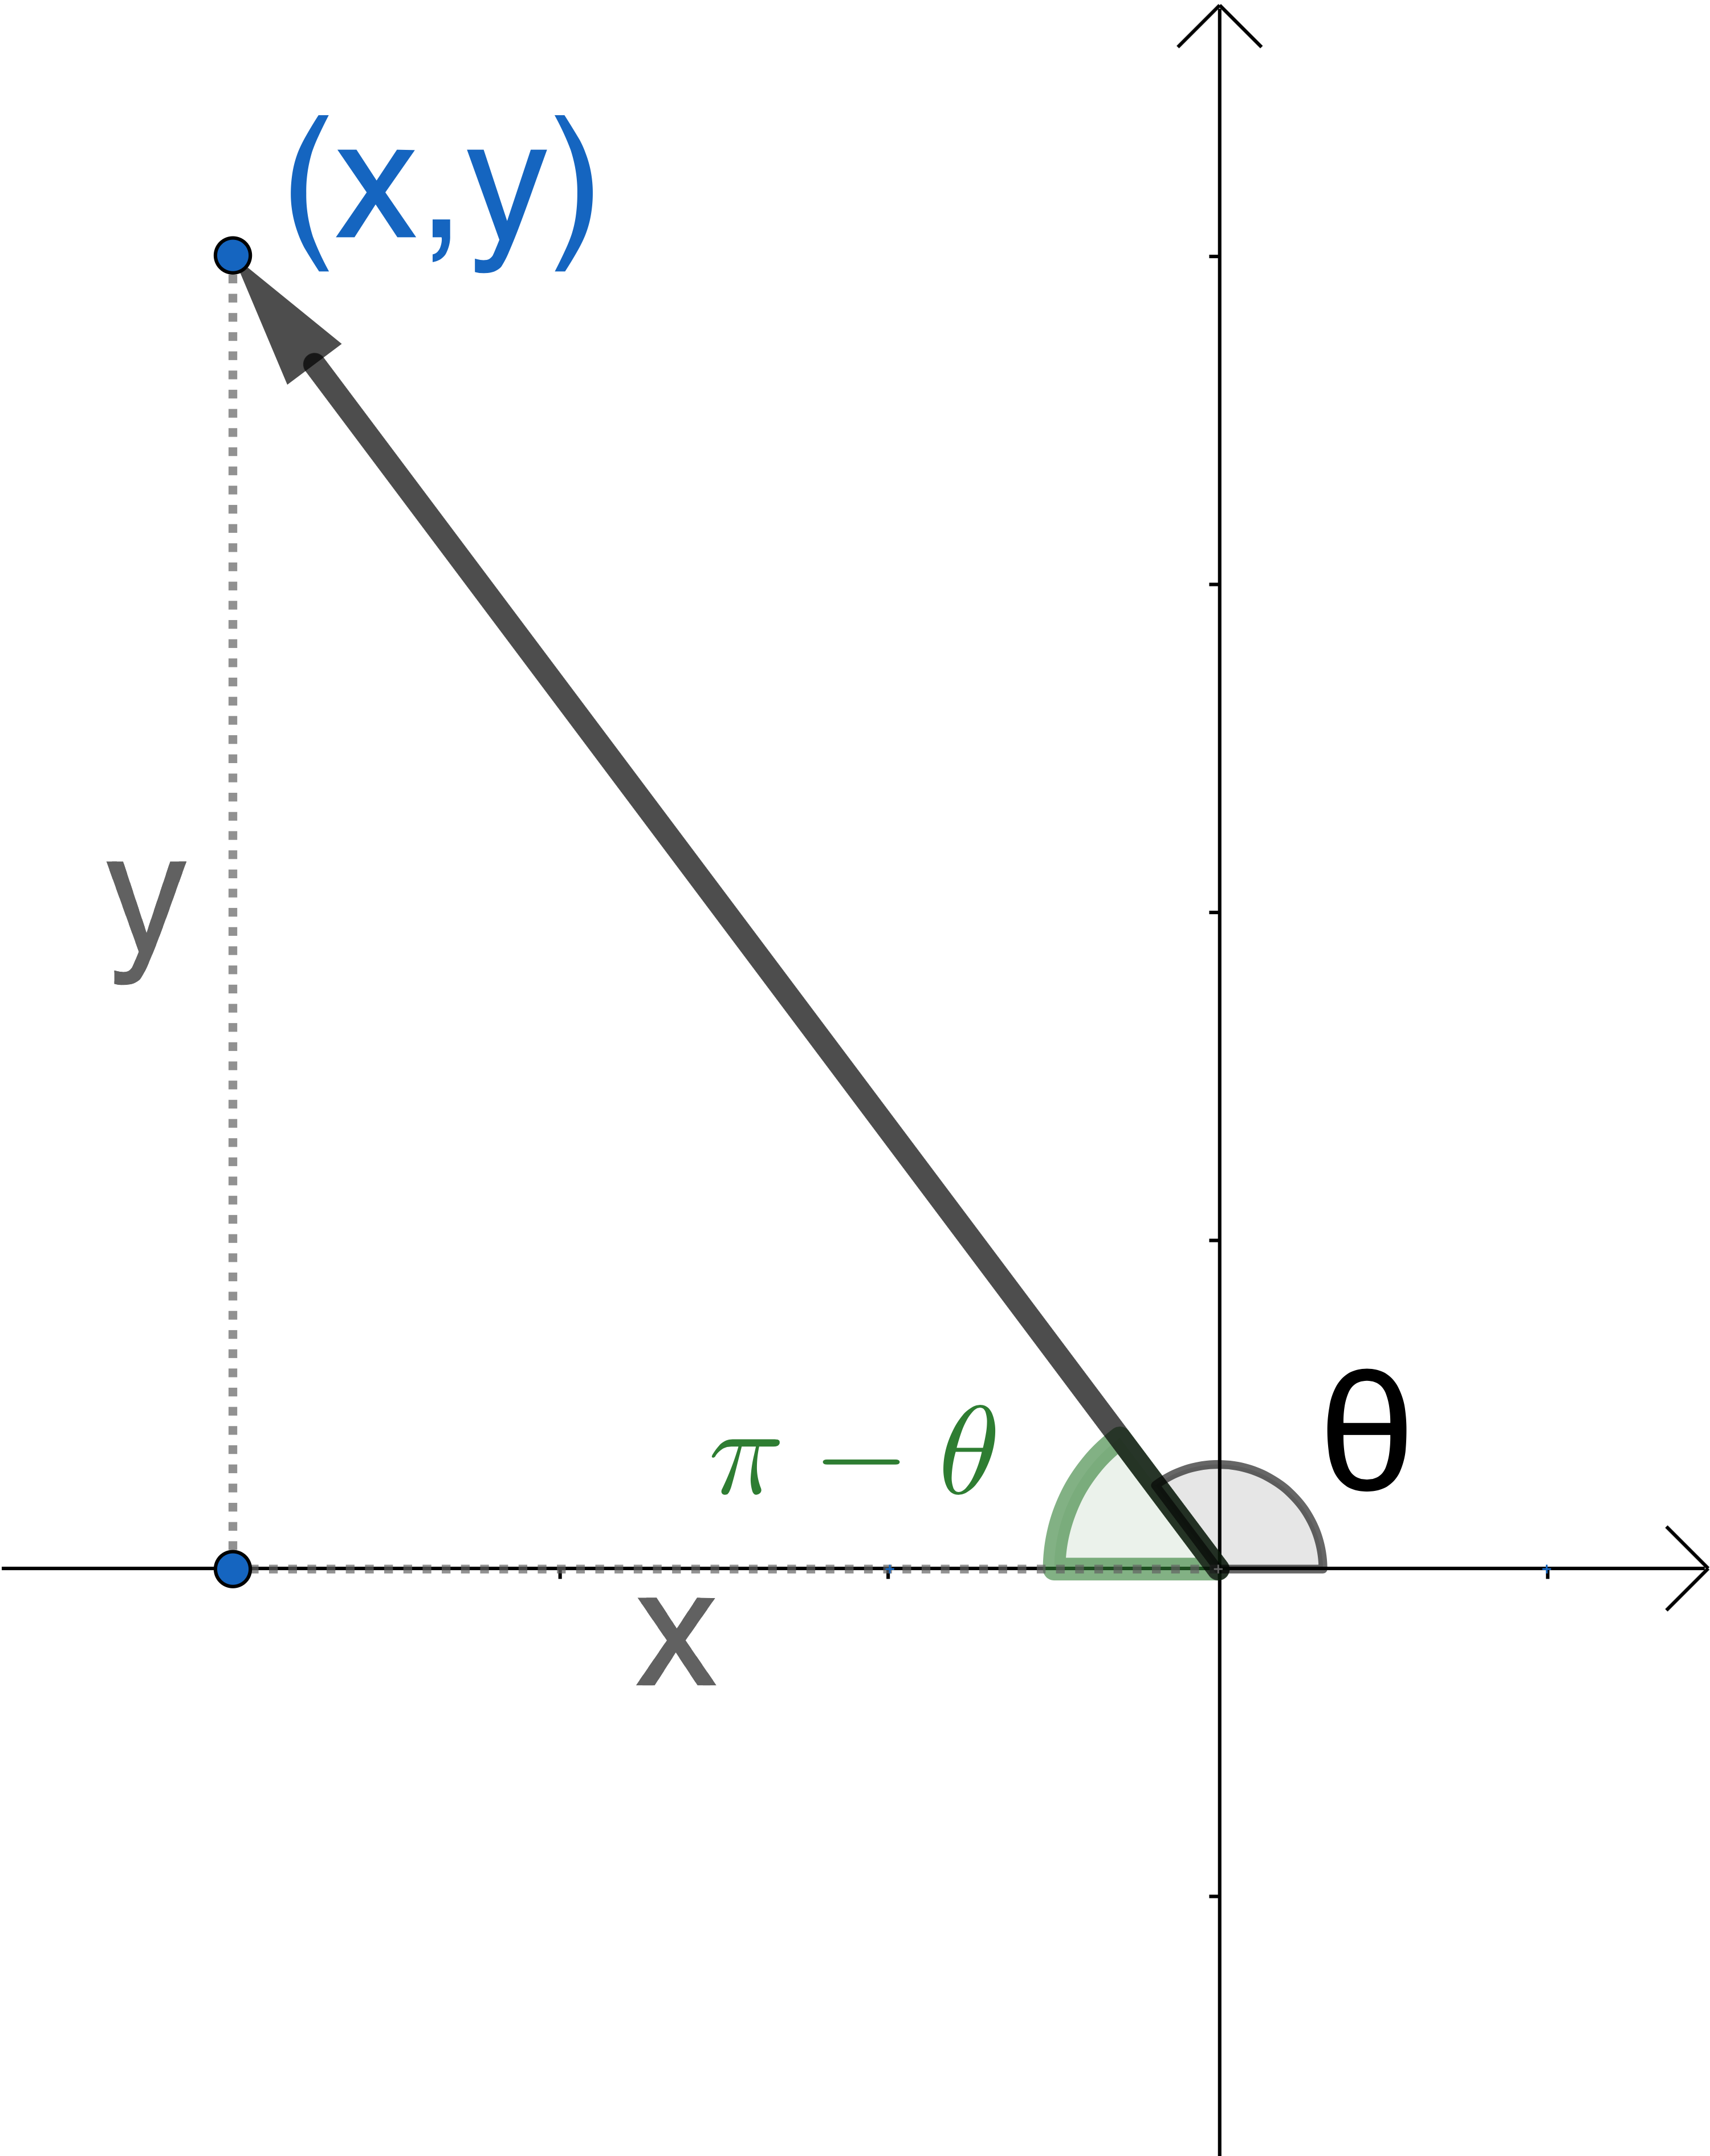
\includegraphics[scale=0.55]{top-left.png}
\column{0.4\textwidth}
If $x<0$ and $y>0$ then
\begin{align*}
\pi-\theta &= \tan^{-1}\left(\frac{y}{|x|}\right)\\
&=\tan^{-1}\left(\frac{y}{-x}\right)\\
&=-\tan^{-1}\left(\frac{y}{x}\right)\\
\end{align*}
and so
\begin{equation*}
\theta = \tan^{-1}\left(\frac{y}{x}\right)+\pi
\end{equation*}
\end{columns}
\end{frame}

\begin{frame}{Bottom left}
\begin{columns}
\column{0.5\textwidth}
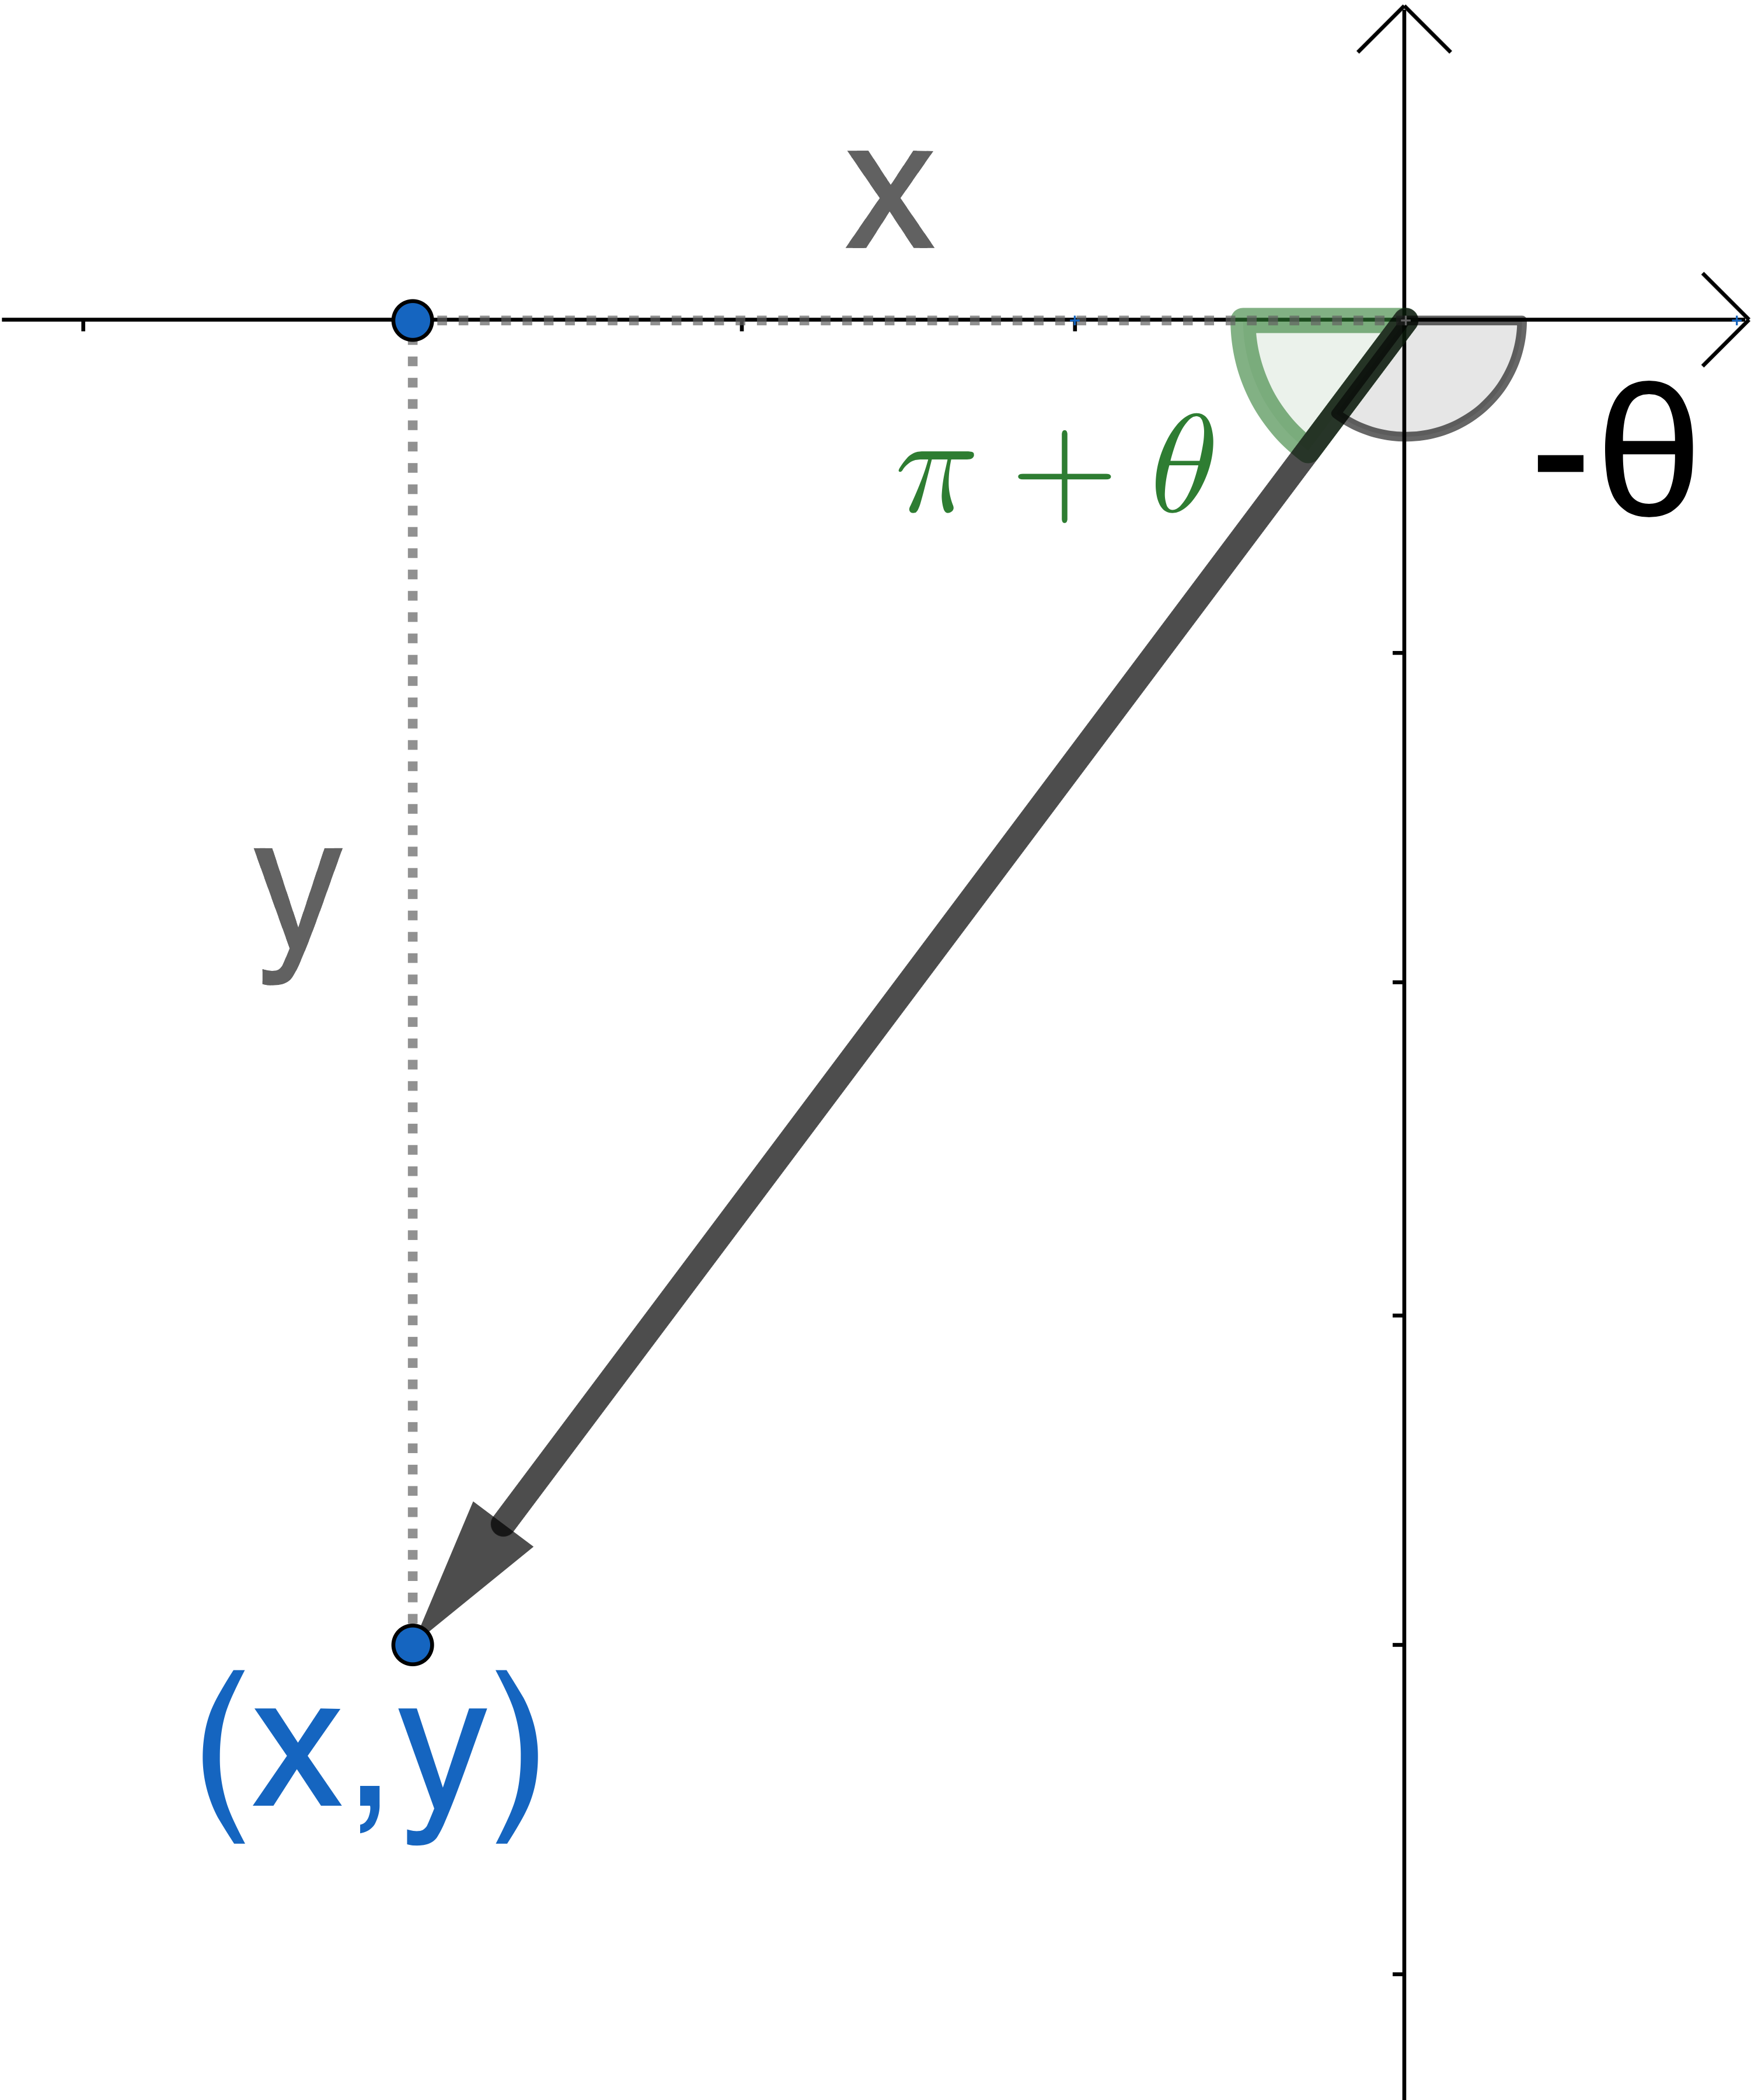
\includegraphics[scale=0.55]{bottom-left.png}
\column{0.4\textwidth}
If $x<0$ and $y<0$ then
\begin{align*}
\pi+\theta &= \tan^{-1}\left(\frac{|y|}{|x|}\right)\\
&=\tan^{-1}\left(\frac{-y}{-x}\right)\\
&=\tan^{-1}\left(\frac{y}{x}\right)\\
\end{align*}
and so
\begin{equation*}
\theta = \tan^{-1}\left(\frac{y}{x}\right)-\pi
\end{equation*}
\end{columns}
\end{frame}

\begin{frame}{Special cases}
\begin{itemize}
	\item If $x=0$ and $y>0$ then $\theta = \frac{\pi}{2}$.\vfill
	\item If $x=0$ and $y<0$ then $\theta = \frac{-\pi}{2}$.\vfill
	\item If $x=0$ and $y=0$ then $\theta$ is undefined.\vfill
	\item If $x<0$ and $y=0$ then $\theta = \pi$.
\end{itemize}
\end{frame}

\begin{frame}{Relationship to complex numbers}
Converting between polar and Cartesian forms gives an alternative representation of a complex number:
\begin{equation*}
x+iy \leftrightarrow R\cos\theta + R\sin\theta i
\end{equation*}
\begin{theorem}[Euler formula]
\begin{equation*}
e^{\theta i} = \cos\theta + \sin\theta i
\end{equation*}
\end{theorem}
and so every complex number can be written as:
\begin{equation*}
x+iy \leftrightarrow R\cdot e^{\theta i}
\end{equation*}
the LHS is called \emph{standard form} and the RHS \emph{polar form}.
\end{frame}

\begin{frame}{Questions?}
Questions?
\end{frame}

\begin{frame}{Examples}
\begin{example}
Convert the following to polar form:-
\begin{itemize}
	\item $-2+2\sqrt{3}i$ % ANS: 4e^{i*2*pi/3}
	\item $3i$ % ANS: 3e^{i*pi/2}
	\item $-1-i$ % ANS: sqrt{2}e^{i*5*pi/4}
	\item $\sqrt{3}+3i$ % ANS: 2*sqrt(3)e^{i*pi/3}
\end{itemize}
\end{example}
\begin{example}
Convert the following to standard form:-
\begin{itemize}
	\item $2e^{\frac{2\pi i}{3}}$ % ANS: -1+sqrt(3)i
	\item $3e^{-i\pi}$ % ANS: -3
	\item $2e^{\frac{3i\pi}{4}}$ % ANS: -sqrt{2}=sqrt{2}i
\end{itemize}
\end{example}
\end{frame}

\section{Multiplication}

\begin{frame}
\begin{beamercolorbox}[sep=12pt,center]{part title}
\usebeamerfont{section title}
\insertsection\par
\end{beamercolorbox}
\end{frame}

\begin{frame}{Graphical interpretation of complex numbers}
If we multiply $z=Re^{i\theta}$ and $w=Qe^{i\phi}$:
\begin{equation*}
zw=Re^{i\theta}Qe^{i\phi} = (RQ)e^{i(\theta+\phi)}
\end{equation*}\vfill
{\bf Slogan:} To multiply two complex numbers we multiply the moduli and add the angles.\vfill
\begin{theorem}[De Moivre Theorem]
\begin{equation*}
(\cos\theta+i\sin\theta)^n = (e^{i\theta})^n = e^{in\theta} = \cos(n\theta)+i\sin(n\theta)
\end{equation*}
\end{theorem}
\end{frame}

\begin{frame}{Questions?}
Questions?
\end{frame}


\begin{frame}{Examples}
\begin{example}
Express $(1-i)^6(\sqrt{3}+i)^3$ in the form $a+bi$. % ANS: -64
\end{example}
\begin{example}
Express $(\frac{1}{2}-\frac{\sqrt{3}}{2}i)^{17}$ in the form $a+bi$. % ANS: 1/2 + (sqrt{3}/2)i
\end{example}
\end{frame}

\section{Complex roots}

\begin{frame}
\begin{beamercolorbox}[sep=12pt,center]{part title}
\usebeamerfont{section title}
\insertsection\par
\end{beamercolorbox}
\end{frame}

\begin{frame}{Principal roots}
If $w = Re^{i\theta}$ then one solution to the equation
\begin{equation*}
z^n = w
\end{equation*}
is 
\begin{equation*}
z = \sqrt[n]{R}\cdot e^{\frac{i\theta}{n}}
\end{equation*}
although there will in fact be $n-1$ more solutions.
\end{frame}

\begin{frame}{Square roots}
\begin{columns}
\column{0.5\textwidth}
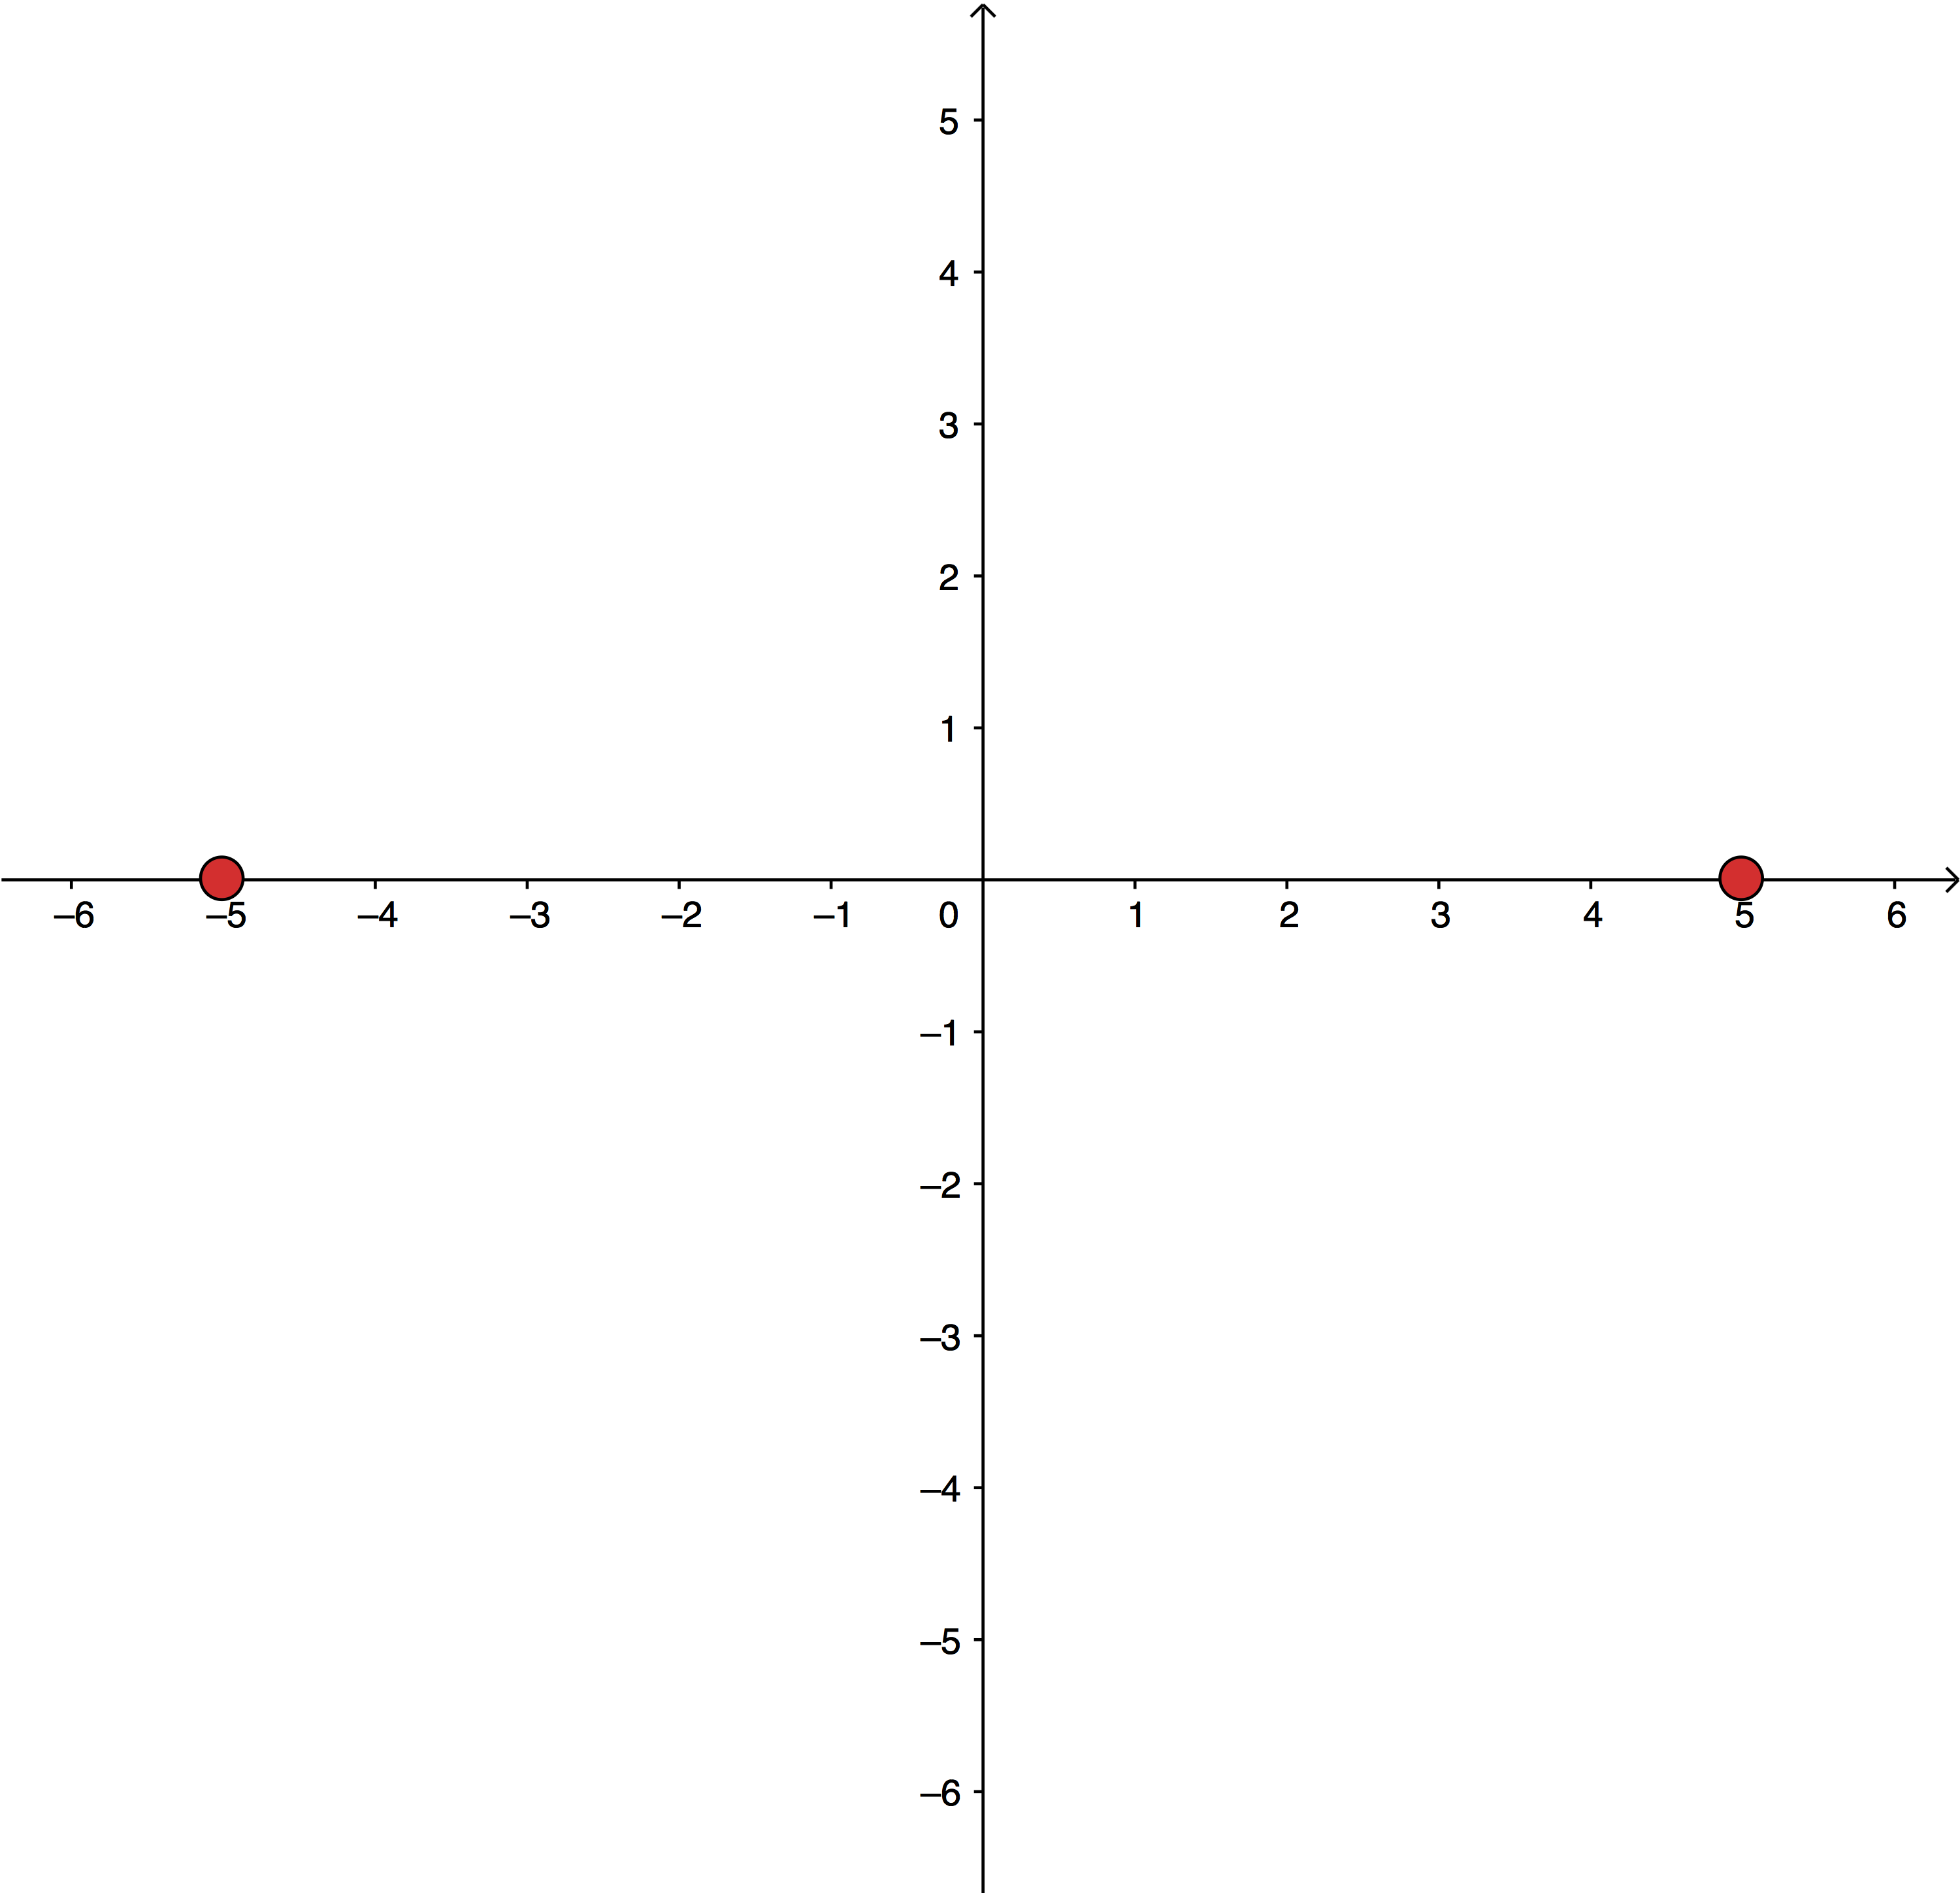
\includegraphics[scale=0.4]{root-25.png}
\column{0.4\textwidth}
The solutions to
\begin{equation*}
	z^2 = 25
\end{equation*}
are
\begin{equation*}
z=+5\text{ and } z=-5
\end{equation*}
\end{columns}
\end{frame}

\begin{frame}{Square roots}
\begin{columns}
\column{0.5\textwidth}
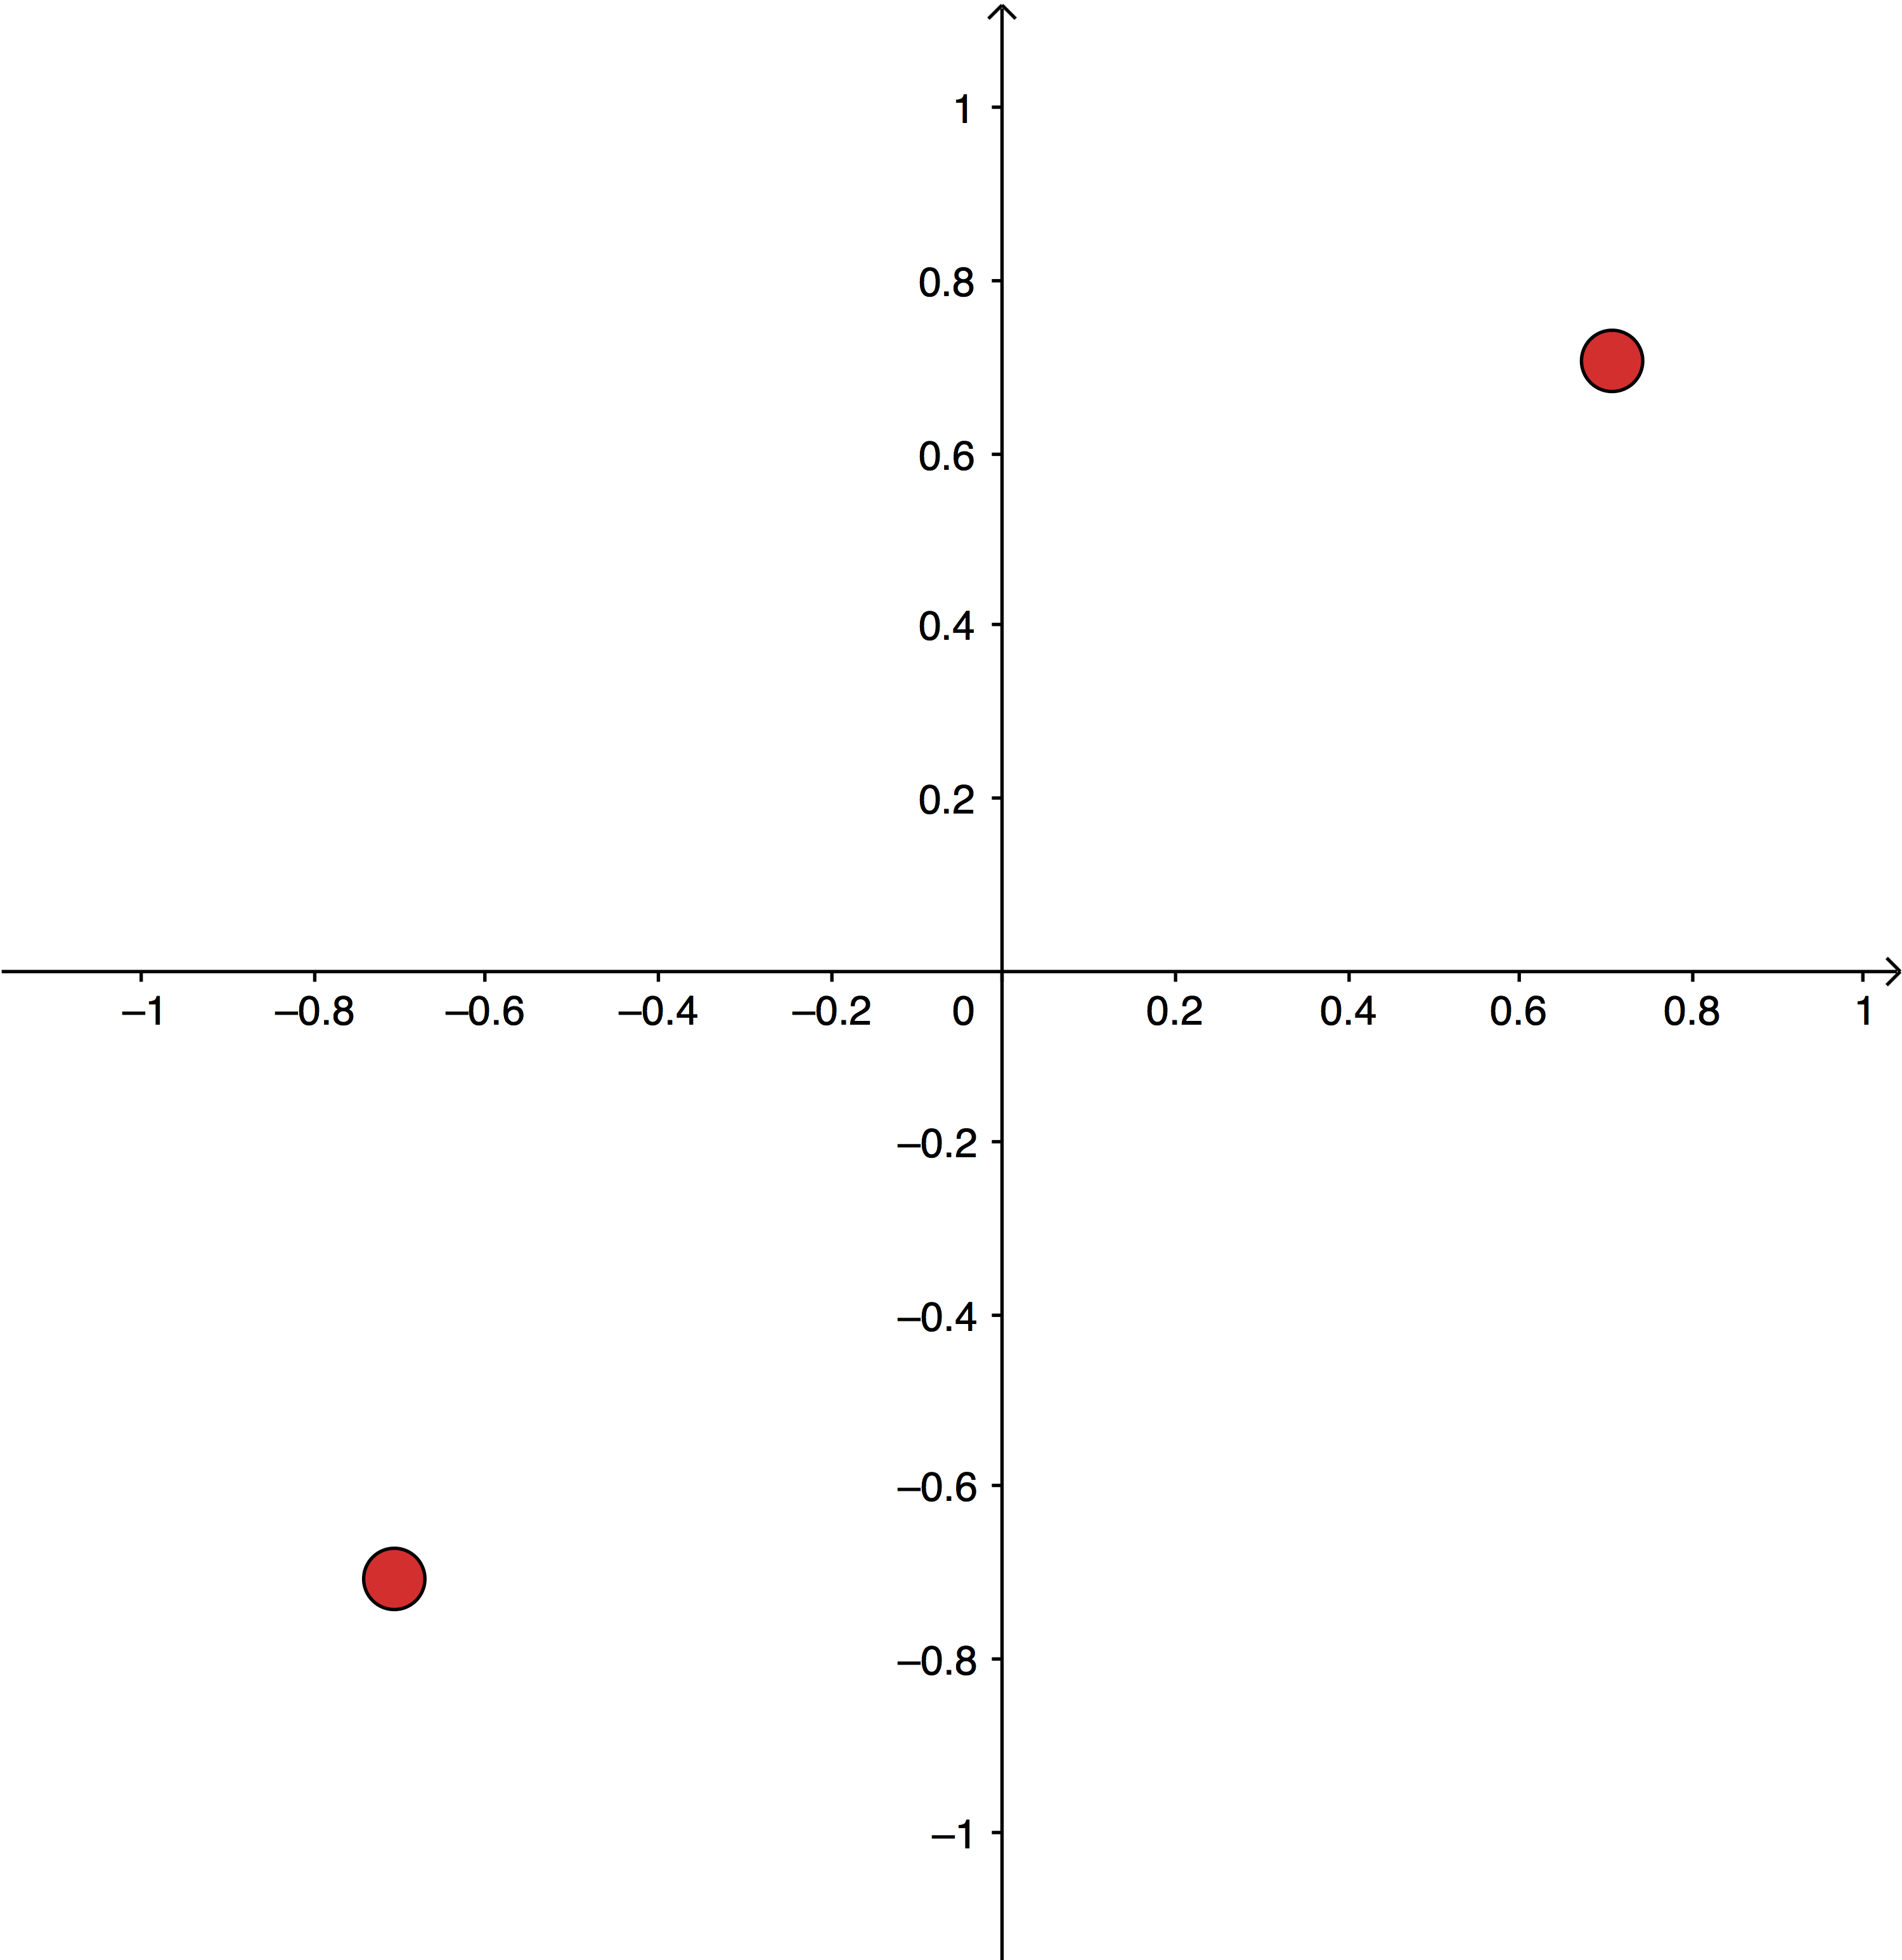
\includegraphics[scale=2.8]{root-i.png}
\column{0.4\textwidth}
The solutions to
\begin{equation*}
	z^2 = i
\end{equation*}
are
\begin{equation*}
z=e^{\frac{\pi}{4}}\text{ and } z=e^{\frac{-3\pi i}{4}}
\end{equation*}
\end{columns}
\end{frame}

\begin{frame}{Square roots}
In general if $w = Re^{i\theta}$ then all of
\begin{equation*}
\sqrt{R}e^{i\left(\frac{\theta}{2}+k\pi\right)}
\end{equation*}
will be square roots of $w$ because
\begin{equation*}
\left(\sqrt{R}e^{i\left(\frac{\theta}{2}+k\pi\right)}\right)^2 = Re^{i\left(\theta+2k\pi\right)} = Re^{i\theta}
\end{equation*}
and then we need to find the values of 
\begin{equation*}
\frac{\theta}{2}+k\pi
\end{equation*}
that are between $-\pi$ and $+\pi$.
\end{frame}

\begin{frame}{Questions?}
Questions?
\end{frame}

\begin{frame}{Examples}
\begin{example}
Find all solutions to the following equations:
\begin{itemize}
	\item $z^2 = 25$. % ANS: -5 and +5
	\item Find all solutions to $z^2 = -1$ % ANS: i and -i
	\item Find all solutions to $z^2 = e^{\frac{i\pi}{4}}$ % ANS: e^{i*pi/8} and e^{-7*i*pi/8}
	\item Find all solutions to $z^3 = i$. (Write in Cartesian form.) % ANS: sqrt(3)/2 + 1/2 i and -i and -sqrt(3)/2 + 1/2 i
	\item Find all solutions to $z^4 = 2(\sqrt{3}i-1)$. (Write in Cartesian form.) % ANS: sqrt{6}/2 + sqrt{2}/2i and + -sqrt{2}/2 +sqrt{6}/2 i and -sqrt{6}/2 - sqrt{2}/2i and  + sqrt{2}/2 -sqrt{6}/2 i
\end{itemize}
\end{example}
\begin{example}
Find all sixth roots of unity.
\end{example}
\end{frame}

\end{document}